\documentclass{article}

\PassOptionsToPackage{numbers, compress}{natbib}

\usepackage{subfig}
\usepackage[utf8]{inputenc} % allow utf-8 input
\usepackage[T1]{fontenc}    % use 8-bit T1 fonts
% \usepackage{hyperref}       % hyperlinks
\usepackage{url}            % simple URL typesetting
\usepackage{booktabs}       % professional-quality tables
\usepackage{amsfonts}       % blackboard math symbols
\usepackage{nicefrac}       % compact symbols for 1/2, etc.
\usepackage{microtype}      % microtypography
\usepackage{xcolor}    
\usepackage{color, colortbl}% colors
\usepackage{algorithm}
\usepackage{algorithmic}
% \usepackage{algpseudocode}
\usepackage[pdftex]{graphicx}
\usepackage{appendix}
\usepackage{multirow}
\usepackage{amsmath}
\usepackage{comment}
\usepackage[colorlinks]{hyperref} 
\usepackage{xcolor}
\usepackage{xspace}
\usepackage{enumitem}
\usepackage[normalem]{ulem}

\renewcommand{\algorithmiccomment}[1]{\hfill $\triangleright$ #1}

\definecolor{LightCyan}{rgb}{0.88,1,1}

% hyperlinks
\hypersetup{colorlinks,allcolors=[rgb]{0.6,0.15,0.00098}}

\newcommand{\chen}[1]{{\color{cyan}{#1}}}
\newcommand{\haotian}[1]{{\color{red}{#1}}}
\newcommand{\alex}[1]{{\color{blue}{\textbf{alex}: #1}}}

\newcommand{\ie}{\textit{i.e.}\xspace}
\newcommand{\eg}{\textit{e.g.}\xspace}
\DeclareMathOperator*{\argmax}{arg\,max}
\DeclareMathOperator*{\argmin}{arg\,min}

% if you need to pass options to natbib, use, e.g.:
%     \PassOptionsToPackage{numbers, compress}{natbib}
% before loading neurips_2023


% ready for submission
\usepackage[final]{neurips_2024}


% to compile a preprint version, e.g., for submission to arXiv, add add the
% [preprint] option:
%     \usepackage[preprint]{neurips_2023}


% to compile a camera-ready version, add the [final] option, e.g.:
%     \usepackage[final]{neurips_2023}


% to avoid loading the natbib package, add option nonatbib:
%    \usepackage[nonatbib]{neurips_2023}


\usepackage[utf8]{inputenc} % allow utf-8 input
\usepackage[T1]{fontenc}    % use 8-bit T1 fonts
\usepackage{hyperref}       % hyperlinks
\usepackage{url}            % simple URL typesetting
\usepackage{booktabs}       % professional-quality tables
\usepackage{amsfonts}       % blackboard math symbols
\usepackage{nicefrac}       % compact symbols for 1/2, etc.
\usepackage{microtype}      % microtypography
\usepackage{xcolor}         % colors



\title{Pixel is a Barrier: Diffusion Models Are More Adversarially Robust Than We Think}


% The \author macro works with any number of authors. There are two commands
% used to separate the names and addresses of multiple authors: \And and \AND.
%
% Using \And between authors leaves it to LaTeX to determine where to break the
% lines. Using \AND forces a line break at that point. So, if LaTeX puts 3 of 4
% authors names on the first line, and the last on the second line, try using
% \AND instead of \And before the third author name.


\author{%
  Haotian Xue \\
  Georgia Institute of Technology\\
  htxue.ai@gatech.edu\\
  \And
   Yongxin Chen\\
  Georgia Institute of Technology\\
  yongchen@gatech.edu\\
}


\begin{document}


\maketitle


\begin{abstract}

% Adversarial examples for diffusion models are widely used as solutions for safety concerns. By adding adversarial perturbations to personal images, attackers can not edit or imitate them easily. However, it is essential to note that all these protections target the latent diffusion model (LDMs), the adversarial examples for diffusion models in the pixel space (PDMs) are largely overlooked. This may mislead us to think that the diffusion models are vulnerable to adversarial attacks like most deep models. In this paper, we show novel findings that: even though gradient-based white-box attacks can be used to attack the LDMs, they fail to attack PDMs. This finding is supported by extensive experiments of almost a wide range of attacking methods on various PDMs and LDMs with different model structures, meaning diffusion models are much more robust against adversarial attacks. Moreover, we find that PDMs can be used as an off-the-shelf purifier to effectively remove the adversarial patterns that were generated on LDMs to protect the images, which means that most protection methods nowadays, to some extent, cannot protect our images from malicious attacks. We hope that our insights will inspire the community to rethink the adversarial samples for diffusion models as protection methods and move forward to more effective protection. Codes are available in \url{https://github.com/xavihart/PDM-Pure}.

Diffusion models have demonstrated an impressive capability to edit or imitate images, which has raised concerns regarding the safeguarding of intellectual property. To address these concerns, the adoption of adversarial attacks, which introduce adversarial perturbations into protected images, has proven successful. Consequently, diffusion models, like many other deep network models, are believed to be susceptible to adversarial attacks. However, in this work, we draw attention to an important oversight in existing research, as all previous studies have focused solely on attacking latent diffusion models (LDMs), neglecting adversarial examples for diffusion models in the pixel space (PDMs). Through extensive experiments, we demonstrate that nearly all existing adversarial attack methods designed for LDMs fail when applied to PDMs. We attribute the vulnerability of LDMs to their encoders, indicating that diffusion models exhibit strong robustness against adversarial attacks. Building upon this insight, we propose utilizing PDMs as an off-the-shelf purifier to effectively eliminate adversarial patterns generated by LDMs, thereby maintaining the integrity of images. Notably, we highlight that most existing protection methods can be easily bypassed using PDM-based purification. We hope our findings prompt a reevaluation of adversarial samples for diffusion models as potential protection methods. Codes are available in \url{https://github.com/xavihart/PDM-Pure}.


% Generative Diffusion Models excel at generating high-quality images however, they can cause safety issues by maliciously editing or mimicking 







\end{abstract}


\section{Introduction}

Generative diffusion models (DMs)~\citep{ddpm,song2020score,ldm} have achieved great success in generating images with high fidelity. However, this remarkable generative capability of diffusion models is accompanied by safety concerns~\cite{zhang2023text}, especially on the unauthorized editing or imitation of personal images such as portraits or individual artworks~\cite{andersen2023,setty2023}.
%
Recent works~\cite{advdm, glaze,salman2023raising, sdsattack, mist-v2, chen2024smoothattack,ahn2024imperceptible, metacloak} show that adversarial samples (adv-samples) for diffusion models can be applied as a protection against malicious editing. Small perturbations generated by conventional methods in adversarial machine learning~\citep{pgd,goodfellow2014fgsm} can effectively fool popular diffusion models such as Stable Diffusion~\cite{ldm} to produce chaotic results when an imitation attempt is made. However, a significantly overlooked aspect is that all the existing works focus on latent diffusion models (LDMs) and the pixel-space diffusion models (PDMs) are not studied. For LDMs, perturbations are not directly introduced to the input of the diffusion models. Instead, they are applied externally and propagated through an encoder. It has been shown that the encoder-decoder of LDMs is vulnerable to adversarial perturbations ~\cite{zhang2023robustness,sdsattack}, which means that the adv-samples for LDMs have a very different mechanism compared with the adv-samples for PDMs. 
Moreover, some existing works~\cite{liang2023mist, salman2023raising} show that combining encoder-specific loss can enhance the adversary, ~\cite{sdsattack} further demonstrating that 
% the gradient of the denoising process is weak and unstable, and 
the encoder is the bottleneck for attacking LDMs. Building upon this observation, in this paper, we draw attention to
rethink existing adversarial attack methods for diffusion models:

\begin{center}
    \textit{Can we generate adversarial examples for PDMs as we did for LDMs?}
\end{center}

% \chen{combine this with the first paragraph before raising our research question} 

% Instead of attacking the diffusion process itself, current adversarial examples for Latent Diffusion Models heavily rely on attacking the encoder: Glaze~\cite{glaze} is built on minimizing the distance between the attacked image and the target image in the latent space defined by the encoder. Additionally, Mist~\cite{liang2023mist} demonstrates the significance of combining the textural loss derived from the encoder to generate better adversarial samples. Moreover, SDS-attack \cite{sdsattack} further investigates that, the gradient of denoising process is weak and unstable, and the real bottleneck of attacking an LDM is attacking the encoder.
%

We address this question by systematically investigating adv-samples for PDMs. We conduct experiments on various LDMs or PDMs with different network architectures (e.g. U-Net~\cite{ddpm} or Transformer~\cite{dit}), different training datasets, and different input resolutions (e.g. 64, 256, 512). Through extensive experiments, we demonstrate that all the existing methods we tested ~\citep{liang2023mist,mist-v2, glaze, sdsattack, chen2024smoothattack, salman2023raising, advdm}, targeting to attack LDMs, fail to generate effective adv-samples for PDMs. This implies that PDMs are more adversarial robust than we think. 

% \chen{this is confusing More importantly, it means that the previous adversarial examples for diffusion models (AdvDM) are, in fact, one special case of adv-samples for LDMs (AdvLDM) only.}

Building on this insight that PDMs are strongly robust against adversarial perturbations, we further propose PDM-Pure, a universal purifier that can effectively remove the protective perturbations of different scales (e.g. Mist-v2~\cite{mist-v2} and Glaze~\cite{glaze}) based on PDMs trained on large datasets. Through extensive experiments, we demonstrate that PDM-Pure achieves way better performance than all baseline methods.

% \chen{no need to mention this in introduction While GrIDPure~\cite{zhao2023can} shows that we can apply diffusion models in different resolutions to purify our image patch-by-patch, they miss that the key is in fact the pixel space, not the resolution.}



% Pixel is a barrier, the original reverse process of PDMs introduces large randomness directly in the pixel space, making the whole system quite robust to be fooled to generate bad samples. Pixel is also a barrier preventing us from achieving real protection using adversarial perturbations since strong PDMs can be utilized to remove the out-of-distribution perturbations~\cite{diff-pgd}. Our work calls for attention to rethink the problem of adv-samples for DM, and also rethink whether adv-samples can protect our images. Our contributions are summarized as follows.

% \begin{enumerate}[parsep=0pt,topsep=0pt,leftmargin=12pt]
%     \item We revist adversarial examples for diffusion models by investigating PDMs, an area that has largely been overlooked in this field. Existing attacks on LDMs \textbf{can not} be applied to attack PDMs, which means that PDMs show superior robustness against adversarial perturbations.
%     \item Based on the new insights, we propose a simple but effective framework to apply strong PDMs as \textbf{a universal purifier} to remove attack-agnostic adversarial perturbations, easily bypassing current protective methods. 
%     \item \chen{is this a contribution?} We emphasize that \textbf{pixel is a barrier}, the community should rethink the adv-samples for DMs and whether current protections based on adv-samples for LDMs, really provide effective protection.
% \end{enumerate}


To summarize, the pixel is a barrier to adversarial attack; the diffusion process in the pixel space makes PDMs much more robust than LDMs. This property of PDMs also makes real protection against the misusage of diffusion models difficult since all the existing protections can be easily purified using a strong PDM. Our contributions are listed below.

\begin{enumerate}[parsep=0pt,topsep=0pt,leftmargin=12pt]
    \item We observe that most existing works on adversarial examples for protection focus on LDMs. Adversarial attacks against PDMs are \textbf{largely overlooked} in this field. 
    \item We fill in the gap in the literature by conducting extensive experiments on various LDMs and PDMs. We discover that all the existing methods \textbf{fail} to attack the PDMs, indicating that PDMs are much more adversarially robust than LDMs.
    \item Based on this novel insight, we propose a simple yet effective framework termed PDM-Pure that applies strong PDMs as \textbf{a universal purifier} to remove attack-agnostic adversarial perturbations, easily bypassing almost all existing protective methods. 

\end{enumerate}



% we made an observation that most of the works focus on LDM, PDMs are not studied

% we test it and find that PDM is much more robust than LDMs 

% PDM-Pure 




\begin{figure}[t]
  \centering
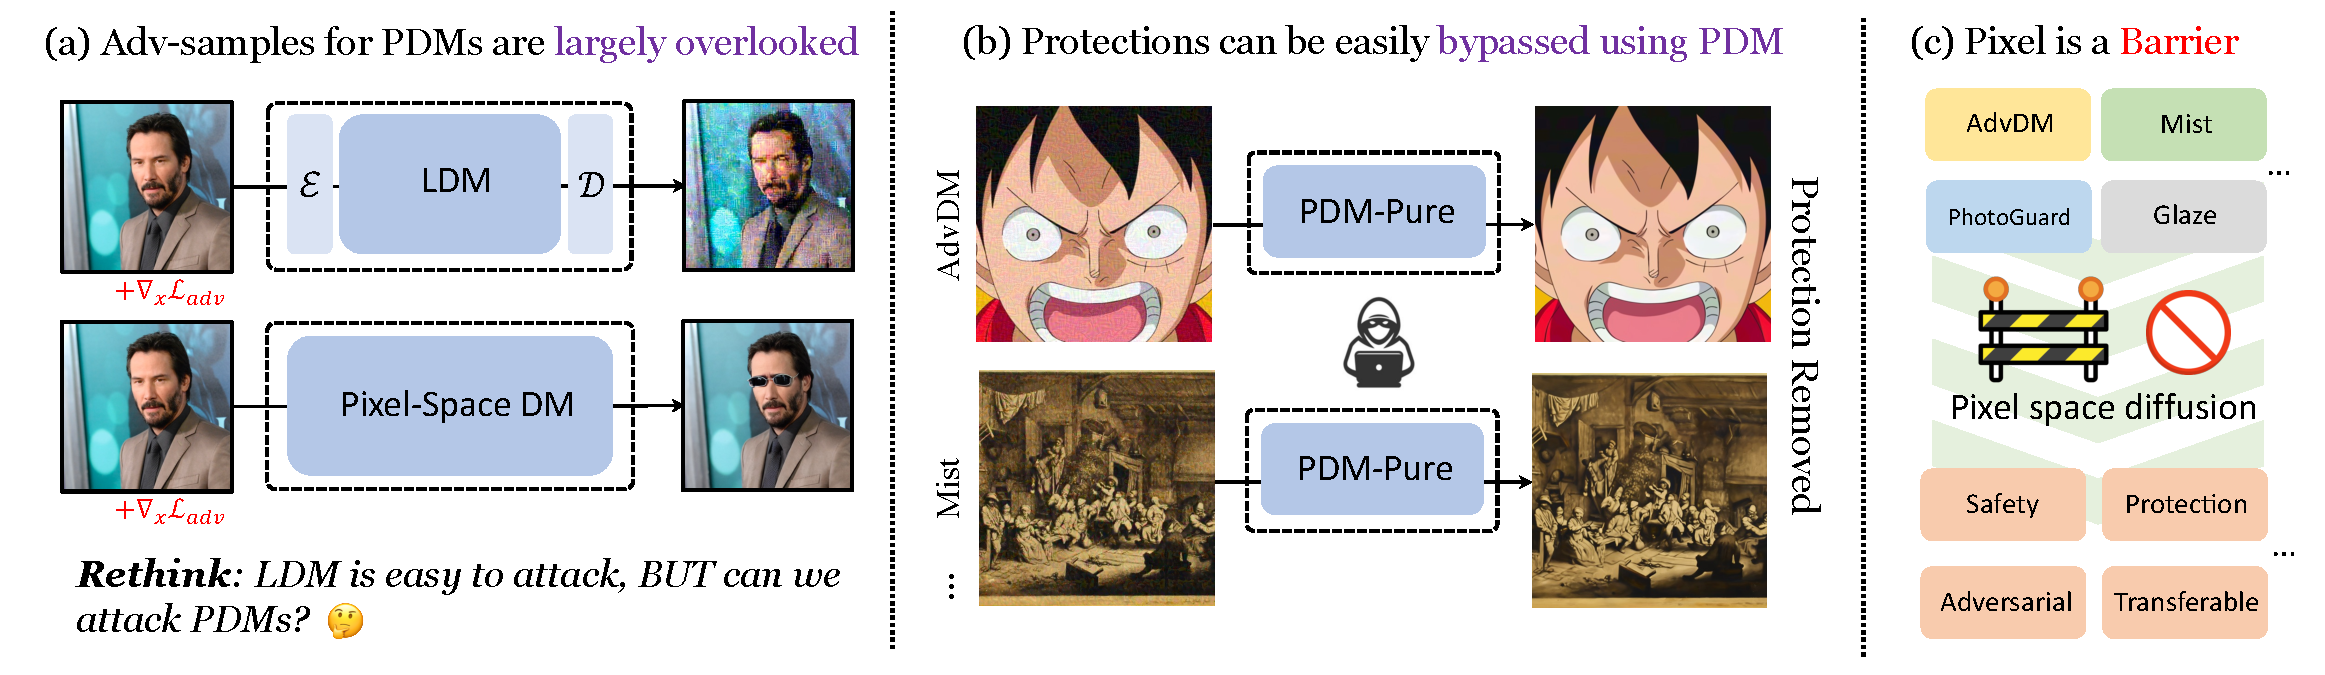
\includegraphics[width=0.99\linewidth]{images/teaser.pdf}
  \vspace{-5pt}
  \caption{\textbf{Pixel is a Barrier for Attacking DMs}: (a) Pixel-based diffusion models are harder to attack using white-box attacks like project-gradient-descent than diffusion models in the latent space. (b) Strong PDM can be used as a universal purifier to effectively remove the protective perturbation generated by existing protection methods. (c) Pixel is a barrier and the pixel-space diffusion model is quite robust, and we cannot achieve real safety and protection if pixel-space diffusion is not attacked. }

  \label{fig:teaser}
  \vspace{-0.4cm}
\end{figure}


% background

% issues


% what we find


%

\section{Related Works}

\paragraph{Safety Issues in Diffusion Models}
The impressive generative capability of the diffusion models has raised numerous safety issues~\cite{zhang2023text,setty2023,andersen2023}. As a result, there has been a growing interest in preventing DMs from being abused. Some of the existing works focus on the protection of intellectual property of diffusion models by applying watermarks~\citep{zhao2023recipe, peng2023protecting, cui2023diffusionshield} and some of them are on concept removal to prevent the DMs from generating NSFW images~\citep{heng2023continual,zhang2023forget,gandikota2023unified}. In the era of generative models, caution should be taken to guarantee safe and responsible applications of these models.

\paragraph{Adversarial Examples for DMs} Adversarial samples~\cite{goodfellow2014fgsm, carlini2017towards, glaze} are clean samples perturbed by an imperceptible small noise that can fool the deep neural networks into making wrong decisions. Under the white-box settings, gradient-based methods are widely used to generate adv-samples. Among them, the projected gradient descent (PGD) algorithm~\cite{pgd} is one of the most effective methods. Recent works~\citep{advdm, salman2023raising} show that it is also easy to find adv-samples for diffusion models (AdvDM): with a proper loss to attack the denoising process, the perturbed image can fool the diffusion models to generate chaotic images when operating diffusion-based mimicry. Furthermore, many improved algorithms~\cite{mist-v2,chen2024smoothattack,sdsattack} have been proposed to generate better AdvDM samples. However, to our best knowledge, all the AdvDM methods listed above are used on LDMs, and those for the PDMs are rarely explored.

\paragraph{Adversarial Perturbation as Protection} Adversarial perturbation against DMs turns out to be an effective method to safeguard images against unauthorized editing~\cite{advdm, glaze,salman2023raising, sdsattack, mist-v2, chen2024smoothattack,ahn2024imperceptible, metacloak}. It has found applications (e.g., Glaze~\cite{glaze} and Mist~\cite{mist-v2, liang2023mist}) for individual artists to protect their creations. SDS-attack~\cite{sdsattack} further investigates the mechanism behind the attack and proposes some tools to make the protection more effective. However, they are limited to protecting LDMs only.
% without further investigating whether they can work for more general PDMs. 
In addition, some works~\cite{zhao2023can, sandoval2023jpeg} find that these protective perturbations can be purified. For instance, GrIDPure~\cite{zhao2023can} find that DiffPure~\cite{nie2022diffusion} can be used to purify the adversarial patterns, but they did not realize that the reason behind this is the robustness of PDMs.


\begin{figure}[t]
  \centering
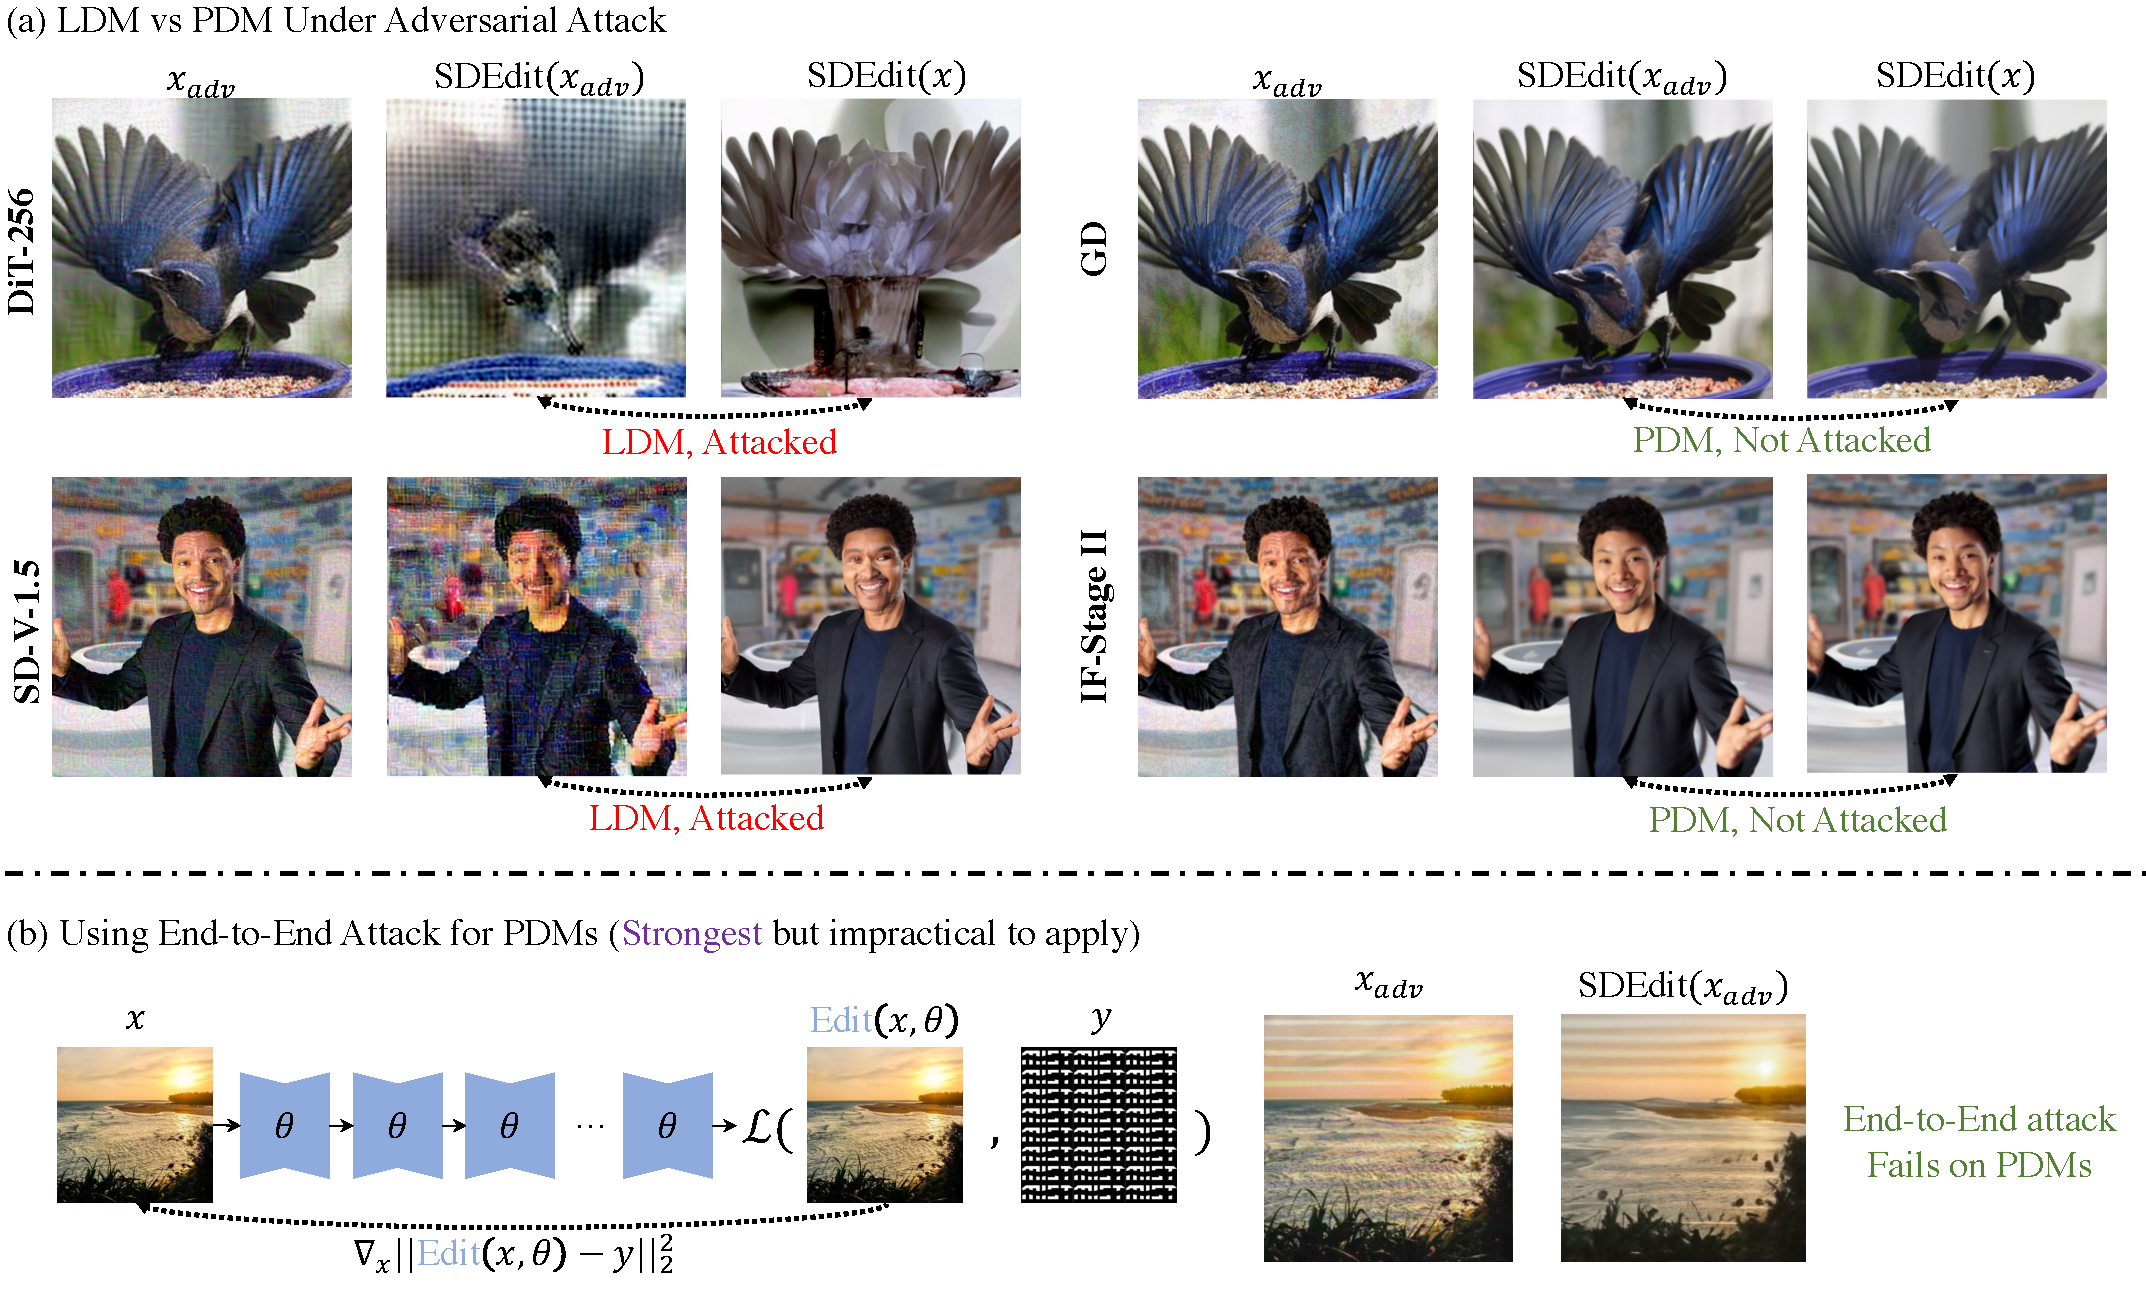
\includegraphics[width=0.99\linewidth]{images/attack.pdf}
  \caption{\textbf{PDMs Cannot be Attacked as LDMs}: (a) LDMs can be easily fooled but PDMs cannot be. (b) Even End-to-End attack does not work on PDMs. (Best viewed with zoom-in)}

  \label{fig:attack_various_models}
  \vspace{-0.4cm}
\end{figure}



\section{Preliminaries}

\paragraph{Generative Diffusion Models}

The generative diffusion model~
\cite{ddpm, song2020score} is one type of generative model, and it has demonstrated remarkable generative capability in numerous fields such as image~\cite{ldm, balaji2022ediffi}, 3D~\cite{poole2022dreamfusion, lin2022magic3d}, video~\cite{vdm,makeavideo}, story~\cite{pan2022story, rahman2023make} and music~\cite{musicdiff, huang2023noise2music} generation. Diffusion models, like other generative models, are parametrized models $p_{\theta}(\hat{x}_0)$ that can estimate an unknown distribution $q(x_0)$. For image generation tasks, $q(x_0)$ is the distribution of real images.

There are two processes involved in a diffusion model, a forward diffusion process and a reverse denoising process. The forward diffusion process progressively injects noise into the clean image, and the $t$-th step diffusion is formulated as $q(x_t \mid x_{t-1} ) = \mathcal{N} (x_t; \sqrt{1 - \beta_t}x_{t-1}, \, \beta_t \mathbf{I})$. Accumulating the noise, we have $    q_t(x_t \mid x_0 ) = \mathcal{N} (x_t; \sqrt{\bar{\alpha}_t} \, x_{t-1}, \, (1-\bar{\alpha}_t) \mathbf{I})$. Here $\beta_t$ growing from $0$ to $1$ are pre-defined values,  $\alpha_t = 1-\beta_t$, and $\bar{\alpha}_t = \Pi_{s=1}^{t} \alpha_s$. Finally, $x_T$ will become approximately an isotropic Gaussian random variable when $\bar{\alpha}_t \rightarrow 0$. 

Reversely, $p_{\theta}(\hat{x}_{t-1}|\hat{x}_{t})$ can generate samples from Gaussian $\hat{x}_T \sim\mathcal{N} (0, \textbf{I})$, where $p_{\theta}$ be re-parameterized by learning a noise estimator $\epsilon_{\theta}$, the training loss is $\mathbb{E}_{t, x_0, \epsilon}[\lambda(t)\|\epsilon_{\theta}(x_t,t) - \epsilon \|^2]$ weighted by $\lambda(t)$, where $\epsilon$ is the noise used to diffuse $x_0$ following $q_t(x_t|x_0)$. Finally, by iteratively applying $p_{\theta}(\hat{x}_{t-1}|\hat{x}_{t})$, we can sample realistic images following $p_{\theta}(\hat{x}_0)$.


Since the above diffusion process operates directly in the pixel space, we call such diffusion models Pixel-Space Diffusion Models (PDMs). Another popular choice is to move the diffusion process into the latent space to make it more scalable, resulting in the Latent Diffusion Models (LDMs)~\cite{ldm}. More specifically, LDMs first use an encoder $\mathcal{E}_{\phi}$ parameterized by $\phi$ to encode $x_0$ into a latent variable $z_0 = \mathcal{E}_{\phi}(x_0)$. The denoising diffusion process is the same as PDMs. At the end of the denoising process, $\hat{z}_0$ can be projected back to the pixel space using decoder $\mathcal{D}_{\psi}$ parameterized by $\psi$ as $\hat{x}_0 = \mathcal{D}_{\psi}(\hat{z}_0)$.

% \chen{breifly introduce SDEdit?}






\begin{table}[t]
 
  \label{tab:my_label}
 \resizebox{\textwidth}{!}{%
  \centering
  \begin{tabular}{c|ccc|ccc|ccc|ccc|c}
  \toprule
    \multicolumn{1}{c}{Models} & 
    \multicolumn{3}{c}{\textbf{FID-score}$\uparrow$} & \multicolumn{3}{c}{\textbf{SSIM} $\downarrow$} & \multicolumn{3}{c}{\textbf{LPIPS} $\uparrow$} & \multicolumn{3}{c}{\textbf{IA-Score} $\downarrow$}  & \textbf{Type} \\
    \midrule
  $\delta=4/255$ & Clean & Adv & $\Delta$  & Clean & Adv & $\Delta$  & Clean & Adv & $\Delta$ & Clean & Adv & $\Delta$ &   \\  

    \midrule
DiT-256 & 131 & 167  & {\color{red}+36}  & 0.37 & 0.35 & {\color{red}-0.02} & 0.44 & 0.54 & {\color{red}+0.10} & 0.74 & 0.70 & {\color{red}-0.04} & LDM  \\
SD-V-1.4 & 44 & 114  & {\color{red}+70}  & 0.68 & 0.55 & {\color{red}-0.13}  & 0.22 & 0.46 & {\color{red}+0.24}  & 0.92 & 0.84 & {\color{red}-0.08}  & LDM  \\
SD-V-1.5 & 45 & 113 & {\color{red}+68}  & 0.73 & 0.59 & {\color{red}-0.14} & 0.20 & 0.38 & {\color{red}+0.138} & 0.94 & 0.89 & {\color{red}-0.05} & LDM  \\
GD-ImageNet & 109 & 109  & +0  & 0.66 & 0.66 & -0.00 & 0.21 & 0.21 & +0.00 & 0.90 & 0.90 & -0.00 & PDM  \\
IF-I & 186 & 187  & +1  & 0.59 & 0.58 & -0.01 & 0.14 & 0.14 & +0.00 & 0.86 & 0.86 & -0.00 & PDM  \\
IF-II & 85 & 87  & +2 & 0.84 & 0.84 & -0.00 & 0.15 & 0.15 & +0.00 & 0.91 & 0.91 & -0.00 & PDM   \\

\midrule
  $\delta=8/255$ & Clean & Adv & $\Delta$  & Clean & Adv & $\Delta$  & Clean & Adv & $\Delta$ & Clean & Adv & $\Delta$ &   \\  

    \midrule
DiT-256 &131 & 186  &{\color{red}+55}  & 0.37 & 0.31 & {\color{red}-0.06} & 0.44 & 0.63 & {\color{red}+0.19} & 0.74 & 0.66 & {\color{red}-0.08} & LDM  \\
SD-V-1.4 & 44 & 178  & {\color{red}+134}  & 0.68 & 0.44 & {\color{red}-0.24}  & 0.22 & 0.60 & {\color{red}+0.38}  & 0.92 & 0.78 & {\color{red}-0.14}  & LDM  \\
SD-V-1.5 & 45 & 179  & {\color{red}+134}  & 0.73 & 0.49 & {\color{red}-0.24} & 0.20 & 0.51 & {\color{red}+0.31} & 0.94 & 0.84 & {\color{red}-0.10} & LDM  \\
GD-ImageNet & 109 & 110  & +1  & 0.66 & 0.64 & -0.02 & 0.21 & 0.22 & +0.01 & 0.90 & 0.90 & -0.00 & PDM  \\
IF-I & 186 & 188  & +2  & 0.59 & 0.59 & -0.00 & 0.14 & 0.14 & +0.00 & 0.86 & 0.86 & +0.00 & PDM  \\
IF-II & 85 & 82   & -3  & 0.84 & 0.83 & -0.01 & 0.15 & 0.16 & +0.01 & 0.91 & 0.92 & +0.01 & PDM   \\






\midrule
  $\delta=16/255$ & clean & adv & $\Delta$  & clean & adv & $\Delta$  & clean & adv & $\Delta$ & clean & adv & $\Delta$ &   \\  

  \midrule
DiT-256 & 131 & 220  & {\color{red}+89}  & 0.37 & 0.26 & {\color{red}-0.11} & 0.44 & 0.70 & {\color{red}+0.26} & 0.74 & 0.63 & {\color{red}-0.11} & LDM  \\
SD-V-1.4 & 44 & 225  & {\color{red}+181}  & 0.68 & 0.34 & {\color{red}-0.34}  & 0.22 & 0.68 & {\color{red}+0.46}  & 0.92 & 0.72 & {\color{red}-0.20}  & LDM  \\
SD-V-1.5 & 45 & 226  & {\color{red}+181}  & 0.73 & 0.37 & {\color{red}-0.36} & 0.20 & 0.62 & {\color{red}+0.42} & 0.94 & 0.78 & {\color{red}-0.16} & LDM  \\
GD-ImageNet & 109 & 110  & +1  & 0.66 & 0.57 & -0.09 & 0.21 & 0.26 & +0.05 & 0.90 & 0.89 & -0.01 & PDM  \\
IF-I & 186 & 188  & +2  & 0.59 & 0.58 & -0.01 & 0.14 & 0.15 & +0.01 & 0.86 & 0.87 & +0.01 & PDM  \\
IF-II &85 & 86  & +1  & 0.84 & 0.76 & -0.08 & 0.15 & 0.21 & +0.06 & 0.91 & 0.95 & +0.04 & PDM   \\


\bottomrule
  \end{tabular}
}
\vspace{10pt}
 \caption{
  \textbf{Quantiative Measurement of PGD-based Adv-Attacks for LDMs and PDMs}: gradient-based diffusion attacks can attack LDMs effectively, making the difference $\Delta$ across all evaluation metrics between edited clean image and edited adversarial image large, which means the quality of edited images drops dramatically (in red). However, the PDMs are not affected much by the crafted adversarial perturbations, showing small $\Delta$ before and after the attacks.
  }
  \label{quant_protect}
  \vspace{-20pt}
\end{table}





\paragraph{Adversarial Examples for Diffusion Models} 
Recent works~\cite{salman2023raising, advdm} find that adding small perturbations to clean images will make the diffusion models perform badly in noise prediction, and further generate chaotic results in tasks like image editing and customized generation. The adversarial perturbations for LDMs can be generated by optimizing the Monte-Carlo-based adversarial loss:

\vspace{-0.4cm}
\begin{equation}\label{semantic_loss}
        \mathcal{L}_{adv}(x) = \mathbb{E}_{t, \epsilon} \mathbb{E}_{z_t \sim q_t(\mathcal{E}_{\phi}(x))}\|\epsilon_{\theta}(z_t, t) -\epsilon \|_2^2.
\end{equation}
\vspace{-0.4cm}

Other encoder-based losses~\cite{glaze, liang2023mist, mist-v2, sdsattack} further enhance the attack to make it more effective. With the carefully designed adversarial loss, we can run Projected Gradient Descent (PGD)~\cite{pgd} with $\ell_{\infty}$ budget $\delta$ to generate adversarial perturbations: 
% \chen{make it clear that $x$ is the clean image}
% \chen{use $x^k$? also $B_\infty(x^k, \delta)$?} \haotian{should be $B_\infty(x, \delta)$, since the budget is computed on the clean sample}

\vspace{-0.4cm}
\begin{equation}\label{pgd_update}    x^{k+1} = \mathcal{P}_{B_\infty(x^0, \delta)} \left[ x^{k} + \eta\, \text{sign}\nabla_{x^k}\mathcal{L}_{adv}(x^k) \right]
\end{equation}

 In the above equation, $\mathcal{P}_{B_\infty(x^0, \delta)}(\cdot)$ is the projection operator on the $\ell_\infty$ ball, where $x^0$ is the clean image to be perturbed. We use superscript $x^k$ to represent the iterations of the PGD and subscript $x_t$ for the diffusion steps. 

    
\begin{figure}[t]
  \centering
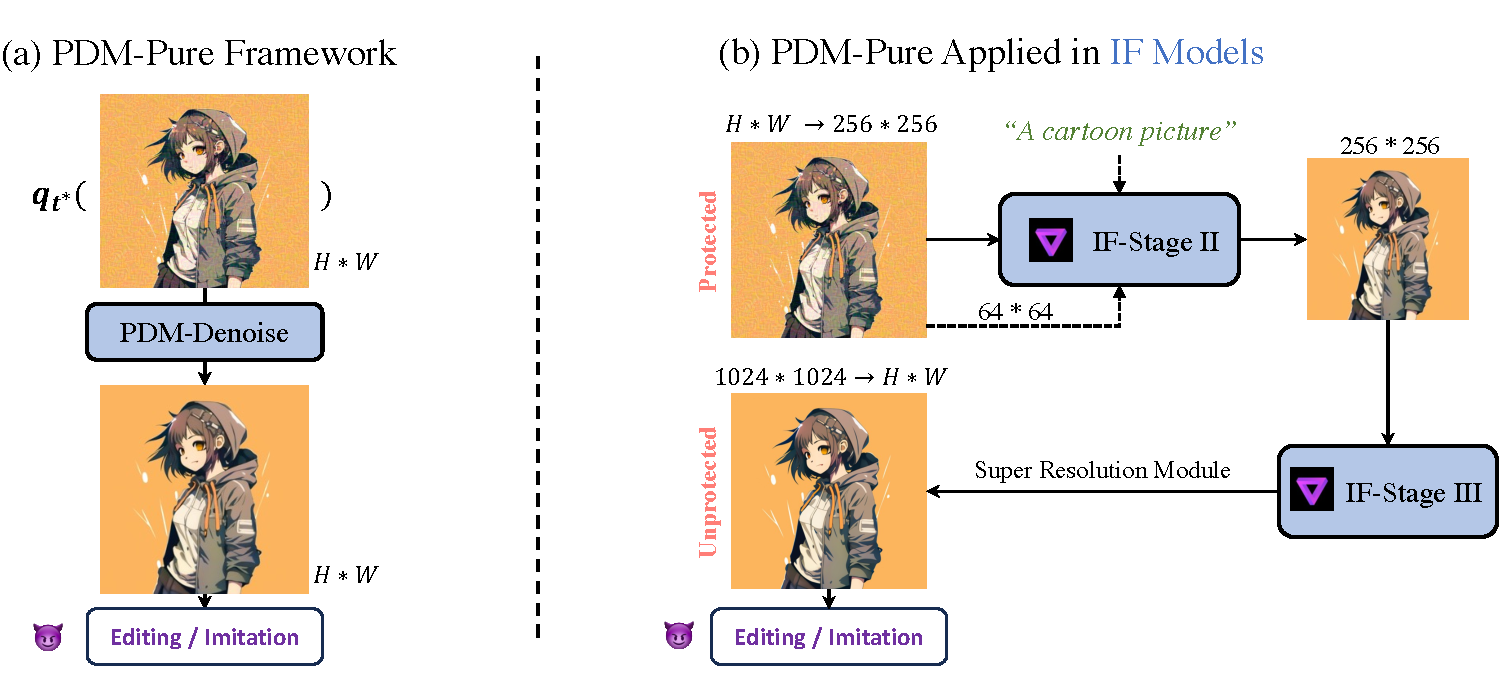
\includegraphics[width=0.8\linewidth]{images/purifier.pdf}
  \vspace{-5pt}
  \caption{\textbf{PDM-Pure is Easy to Design:} (a) PDM-Pure applies SDEdit~\cite{meng2021sdedit} in the pixel space: it first runs forward diffusion with a small step $t^{*}$ and then runs denoising process. (b) We adapt the framework to DeepFloyd-IF~\cite{deepfloyd}, one of the strongest PDMs. PDM-Pure can effectively remove strong protective perturbations (e.g. $\delta=16/255$). The images we tested are sized $512\times 512$.}

\label{fig:purification_pipeline}
  \vspace{-0.5cm}
\end{figure}



\section{Rethink Adversarial Examples for Diffusion Models}

Adversarial examples of LDMs are widely adopted as a protection mechanism to prevent unauthorized images from being edited or imitated~\cite{glaze, liang2023mist}. However, a significant issue overlooked is that all the adversarial examples in existing work are generated using LDMs, primarily due to the wide impact of the Stable Diffusion; no attempts have been made to attack PDMs. 

This lack of investigation may mislead us to conclude that diffusion models, like most deep neural networks, are vulnerable to adversarial perturbations, and that the algorithms used in LDMs can be transferred to PDMs by simply applying the same adversarial loss in the pixel space formulated as:

\vspace{-0.4cm}
\begin{equation}\label{pixel_diffusion_adversarial_loss}
    \mathcal{L}_{adv}(x) = \mathbb{E}_{t, \epsilon} \mathbb{E}_{x_t \sim q_t(x)}\|\epsilon_{\theta}(x_t, t) -\epsilon \|_2^2
\end{equation}

However, we show through experiments that PDMs are robust against this form of attack (Figure~\ref{fig:attack_various_models}), which means all the existing attacks against diffusion models are, in fact, special cases of attacks against the LDMs only.
Prior to this study, there may have been a prevailing belief that diffusion models could be easily deceived. However, our research reveals an important distinction: it is the LDMs that exhibit vulnerability, while the PDMs demonstrate significantly higher adversarial robustness.
% Before this work, people may think that diffusion models can be easily fooled, but the truth is that only LDMs are, the original PDMs are much more adversarially robust. 
We conduct extensive experiments on popular LDMs and PDMs structures including DiT, Guided Diffusion, Stable Diffusion, and DeepFloyd, and demonstrate in Table~\ref{quant_protect} that only the LDMs can be attacked and PDMs are not that susceptible to adversarial perturbations. More details and analysis can be found in the experiment section.



The vulnerability of the LDMs is caused by the vulnerability of the latent space~\cite{sdsattack}, meaning that although we may set budgets for perturbations in the pixel space, the perturbations in the latent space can be large. In~\cite{sdsattack}, the authors show statistics of perturbations in the latent space over the perturbations in the pixel space and this value $\frac{|\delta_z|}{|\delta_x|}$ can be as large as $10$. In contrast, the PDMs directly work in the pixel space, and thus the injected noise combined with the random Gaussian noise will not easily fool the denoiser as it is trained to be robust to Gaussian noise of different levels. 








Almost all the copyright protection perturbations~\cite{glaze, liang2023mist, mist-v2} are based on the insight that it is easy to craft adversarial examples to fool the diffusion models.  We need to rethink the adversarial samples of diffusion models since there are a lot of PDMs that cannot be attacked easily. Next, we show that PDMs can be utilized to purify all adversarial patterns generated by existing methods in Section~\ref{sec:pdm_pure}.  This new landscape poses new challenges to ensure the security and robustness of diffusion-based copyright protection techniques.




\section{PDM-Pure: PDM as a Strong  Universal Purifier}~\label{sec:pdm_pure}
\vspace{-0.4cm}

Given the robustness of PDMs, a natural idea emerges: we can utilize PDMs as a universal purification network. This approach could potentially eliminate any adversarial patterns without knowing the nature of the attacks. We term this framework \textbf{PDM-Pure}, which is a general framework to deal with all the perturbations nowadays. To fully harness the capabilities of PDM-Pure, we need to fulfill two basic requirements: (1) The perturbation shows out-of-distribution pattern as reflected in existing works on adversarial purification/attacks using diffusion models~\cite{nie2022diffusion,diff-pgd} (2) The PDM being used is strong enough to represent $p(x_0)$, which can be largely determined by the dataset they are trained on. 

It is \textbf{effortless} to design a PDM-Pure. The key idea behind this method is to run SDEdit in the pixel space. Given any strong pixel-space diffusion model, we add a small noise to the protected images and run the denoising process (Figure~\ref{fig:purification_pipeline}), and then the adversarial pattern should be removed. The key idea of PDM-Pure is simple. In practice, we need to adjust the pipeline to fit the resolution of the PDMs being used. 

Here, we explain in detail how to adapt DeepFloyd-IF~\cite{deepfloyd}, the strongest open-source PDM as far as we know, for PDM-Pure. DeepFloyd-IF is a cascaded text-to-image diffusion model trained on 1.2B text-image pairs from LAION dataset~\cite{schuhmann2022laion}. It contains three stages named IF-Stage I, II, and III. Here we only use Stage II and III since Stage I works in a resolution of $64$ which is too low. Given a perturbed image $x_{W\times H}$ sized $W\times H$, we first resize it into $x_{64\times 64}$ and $x_{256\times 256}$. Then we use a general prompt  $\mathcal{P}$ to do SDEdit~\cite{meng2021sdedit} using the Stage II model: 
% $x_t = \textbf{IF-II}(x_{t+1}, x_{64\times 64}, p)$

\begin{equation}
    x_t = \textbf{IF-II}(x_{t+1}, x_{64\times 64}, \mathcal{P})
\end{equation}

where $t=T_{\text{edit}}-1, ...,1, 0$, $x_{T_{\text{edit}}}=x_{256\times 256}$. A larger $T_{\text{edit}}$ may be used for larger noise. $x_0$ is the purified image we get in the $256\times 256$ resolution space, where the adversarial patterns should be already purified. We can then use IF Stage III to further up-sample it into $1024\times 1024$ with $x_{1024\times 1024} = \textbf{IF-III}(x_0, p)$. Finally, we can sample into $H\times W$ as we want through downsampling. This whole process is demonstrated in Figure~\ref{fig:purification_pipeline}. After purification, the image is no longer adversarial to the targeted diffusion models and can be effectively used in downstream tasks.

In the main paper, we conduct experiments on purifying protected images sized $512\times 512$. For images with a larger resolution, purifying in the resolution of $256\times 256$ may lose information. In Appendix~\ref{supp:section:pdm_pure_for_higher_resolution} we show PDM-Pure can also applied to purify patches of high-resolution inputs.








\begin{table}[t]
 
  \label{tab:my_label}
 \resizebox{\textwidth}{!}{%
  \centering
  \begin{tabular}{ccccccccc}
\toprule
Methods & AdvDM & AdvDM(-) & SDS(-) & SDS(+) & SDST & Photoguard & Mist & Mist-v2 \\

% \midrule

% $\delta=4/255$ \\
% \midrule

% Crop-Resize & 0 & 0 & 0 & 0 & 0 & 0 & 0 & 0\\

% JPEG & 0 & 0 & 0 & 0 & 0 & 0 & 0 & 0\\

% Adv-Clean & 0 & 0 & 0 & 0 & 0 & 0 & 0 & 0\\

% LDM-Pure& 0 & 0 & 0 & 0 & 0 & 0 & 0 & 0\\

% GrIDPure & 0 & 0 & 0 & 0 & 0 & 0 & 0 & 0\\

% PDM-Pure (ours) & 0 & 0 & 0 & 0 & 0 & 0 & 0 & 0\\

% \midrule
% $\delta=16/255$ \\
\midrule

Before Protection & 166 & 166 & 166 & 166 & 166 & 166 & 166 & 166 \\

After Protection & 297 &221 & 231 & 299 & 322 & 375 & 372 & 370 \\

\midrule

Crop-Resize & 210 & 271 & 228 & 217 & 280 & 295 & 289 & 288\\

JPEG & 296 & 222 & 229 & 297 & 320 & 359 & 351 & 348 \\

Adv-Clean & 243 & 201 & 204 & 244 & 243 & 266 & 282 & 270 \\

LDM-Pure& 300 & 251 & 235 & 300 & 350 & 385 & 380 & 375 \\

GrIDPure & 200 & 182 & 195 & 200 & 210 & 220 & 230 & 210 \\
\rowcolor{LightCyan}
PDM-Pure (ours) & \textbf{161} & \textbf{170} & \textbf{165} & \textbf{159} & \textbf{179} & \textbf{175} & \textbf{178} & \textbf{170}\\

\bottomrule
  \end{tabular}

}
\vspace{10pt}
 \caption{
  \textbf{Quantiative Measurement of Different Purification Methods in Different Scale (FID-score)}: We compute the FID-score of editing purified images over the clean dataset. PDM-Pure is the strongest to remove all the tested protection, under strong protection with $\delta=16$. GrIDPure~\cite{zhao2023can} can also do reasonable protection, but the performance is limited because the PDM they used is not strong enough.
  }
  \label{quant_purify}
  \vspace{-0.8cm}
\end{table}

\section{Experiments}

In this section, we conduct experiments on various attacking methods and various models to support the following two conclusions:

\begin{itemize}[parsep=0pt,topsep=0pt,leftmargin=12pt]
    \item \textbf{(C1)}: PDMs are much more adversarial robust than LDMs, and PDMs can not be effectively attacked using all the existing attacks for LDMs.
    \item \textbf{(C2)}: PDMs can be applied to effectively purify all of the existing protective perturbations. Our PDM-Pure based on DeepFloyd-IF shows state-of-the-art purification power.
    % \item \textbf{(C3)}: Pixel is a barrier for us to achieve real protection against diffusion-based mimicry. PDM-Pure can make the protective perturbation no more protective, and there is currently no effective way to attack PDMs.
\end{itemize}

\subsection{Models, Datasets, and Metrics} 
The models we used can be categorized into LDMs and PDMs. For LDMs, we use Stable Diffusion V-1.4, V-1.5 (SD-V-1.4, SD-V-1.5)~\cite{ldm}, and Diffusion Transformer (DiT-XL/2)~\cite{dit}, and for PDMs we use Guided Diffusion (GD)~\cite{guideddiffusion} trained on ImageNet~\cite{deng2009imagenet}, and DeepFloyd Stage I and Stage II~\cite{deepfloyd}. 

For models trained on the ImageNet (DiT, GD), we run adversarial attacks and purification on a 1k subset of the ImageNet validation dataset. For models trained on LAION, we run tests on the dataset proposed in~\cite{sdsattack}, which includes $400$ cartoon, artwork, landscape, and portrait images. The metrics for testing the quality of generated images are included in the Appendix.

For protection methods, we consider almost all the representative approaches, including AdvDM~\cite{advdm}, SDS~\cite{sdsattack}, Mist~\cite{liang2023mist}, Mist-v2~\cite{mist-v2}, Photoguard~\cite{salman2023raising} and Glaze~\cite{glaze}. We also test the methods in the design space proposed in ~\cite{sdsattack}, including  SDS(-), AdvDM(-), and SDST. In contrast to other existing methods, they are based on gradient descent and have shown great performance in deceiving the LDMs.






\subsection{(C1) PDMs are Much More Robust Than We Think} 

In Table~\ref{quant_protect}, we attack different LDMs and PDMs with one of the most popular adversarial loss~\cite{mist-v2} in Equation~\ref{semantic_loss} and Equation~\ref{pixel_diffusion_adversarial_loss}, which can be interpreted as fooling the denoiser using a Monte-Carlo-based loss. Given the attacked samples, we test the SDEdit results on the attacked samples, which can be generally used to test whether the samples are adversarial for the diffusion model or not. We use FID-score~\cite{fid}, SSIM~\cite{ssim}, LPIPS~\cite{lpips}, and IA-Score~\cite{la-score} to measure the quality of the attack. If the quality of generated images decreases a lot compared with editing the clean images, then the attack is successful. We can see that LDMs can be easily attacked, while PDMs are quite robust; the quality of the edited images is still good. We also show some visualizations in Figure~\ref{fig:attack_various_models}, which illustrates that the perturbation will affect the LDMs but not the PDMs.

To further investigate how robust PDM is, we test other advanced attacking methods, including the End-to-End Diffusion Attacks (E2E-Photoguard) proposed in~\cite{salman2023raising} and the Improved Targeted Attack (ITA) proposed in ~\cite{mist-v2}. Though the End-to-End attack is usually impractical to run, it shows the strongest performance to attack LDMs.  We find that both attacks are not successful in PDM settings. We show attacked samples and edited samples in Figure~\ref{fig:attack_various_models} as well as the Appendix. In conclusion, existing adversarial attack methods for diffusion models can only work for the LDMs, and PDMs are more robust than we think.


\subsection{(C2) PDM-Pure: A Universal Purifier that is Simple yet Effective}

PDM-Pure is simple: basically, we just run SDEdit to purify the protected image in the pixel space. Given our assumption that PDMs are quite robust, we can use PDMs trained on large-scale datasets as a universal black-box purifier. We follow the model pipeline introduced in Section~\ref{sec:pdm_pure} and purify images protected by various methods in Table~\ref{quant_purify}.

PDM-Pure is effective: from Table~\ref{quant_purify} we can see that the purification will remove adversarial patterns for all the protection methods we tested, largely decreasing the FID score for the SDEdit task. Also, we test the protected images and purified images in more tasks including Image Inpainting~\cite{song2020score}, Textual-Inversion~\cite{textualinversion}, and LoRA customization~\cite{lora} in Figure~\ref{fig:purification_results}. Both qualitative and quantitative results show that the purified images are no more adversarial and can be effectively edited or imitated in different tasks without any obstruction. 

Also, PDM-Pure shows SOTA results compared with previous purification methods, including some simple purifiers based on compression and filtering like Adv-Clean, crop-and-resize, JPEG Compression, and  SDEdit-based methods like GrIDPure~\cite{zhao2023can}, which uses patchified SDEdit with a GD~\cite{guideddiffusion}. We also add LDM-Pure as a baseline to show that LDMs can not be used to purify the protected images. For GrIDPure, we use Guided-Diffusion trained on ImageNet to run patchified purification. All the experiments are conducted on the datasets collected in ~\cite{sdsattack} under the resolution of $512\times 512$. Results for higher resolutions are presented in Appendix~\ref{supp:section:pdm_pure_for_higher_resolution}.




% \subsection{(C3) Pixel is A Barrier: What Should We Do in the Future?}

% \chen{why is this in the experiment section? Are any experiments involved?} Pixel is a barrier for us to do real protection against adversarial attacks. Since PDMs are quite robust, they cannot be easily attacked and can even be used to purify the protective perturbations, challenging the current assumption for safety protection of generative diffusion models. The community should rethink the problem of adversarial samples for generative diffusion models and rethink can we rely on them to protect unauthorized images. Hence, diffusion models turn out to be quite robust, more research should be conducted to study them and the reason behind them. If the robustness can be verified and guaranteed, we may rely on it as a new structure for many other tasks.\haotian{move it the the conclusion}


\section{Conclusions and Future Directions}


In this paper, we present novel insights that while many studies demonstrate the ease of finding adversarial samples for Latent Diffusion Models (LDMs), Pixel Diffusion Models (PDMs) exhibit far greater adversarial robustness than previously assumed. We are the first to investigate the adversarial samples for PDMs, revealing a surprising discovery that existing attacks fail to fool PDMs. Leveraging this insight, we propose utilizing strong PDMs as universal purifiers, resulting in PDM-Pure, a simple yet effective framework that can generate protective perturbations in a black-box manner. 


Pixel is a barrier for us to do
real protection against adversarial attacks. Since PDMs are quite robust, they cannot be easily attacked.
PDMs can even be used to purify the protective perturbations, challenging the current assumption for
the safe protection of generative diffusion models. We advocate rethinking the problem of
adversarial samples for generative diffusion models and 
unauthorized image protection based on it. 
% Diffusion models turn out to be quite robust, 
More rigorous study can be
conducted to better understand the mechanism behind the robustness of PDMs. Furthermore, we can utilize it as a new structure for many other tasks

\begin{figure}[H]
  \centering
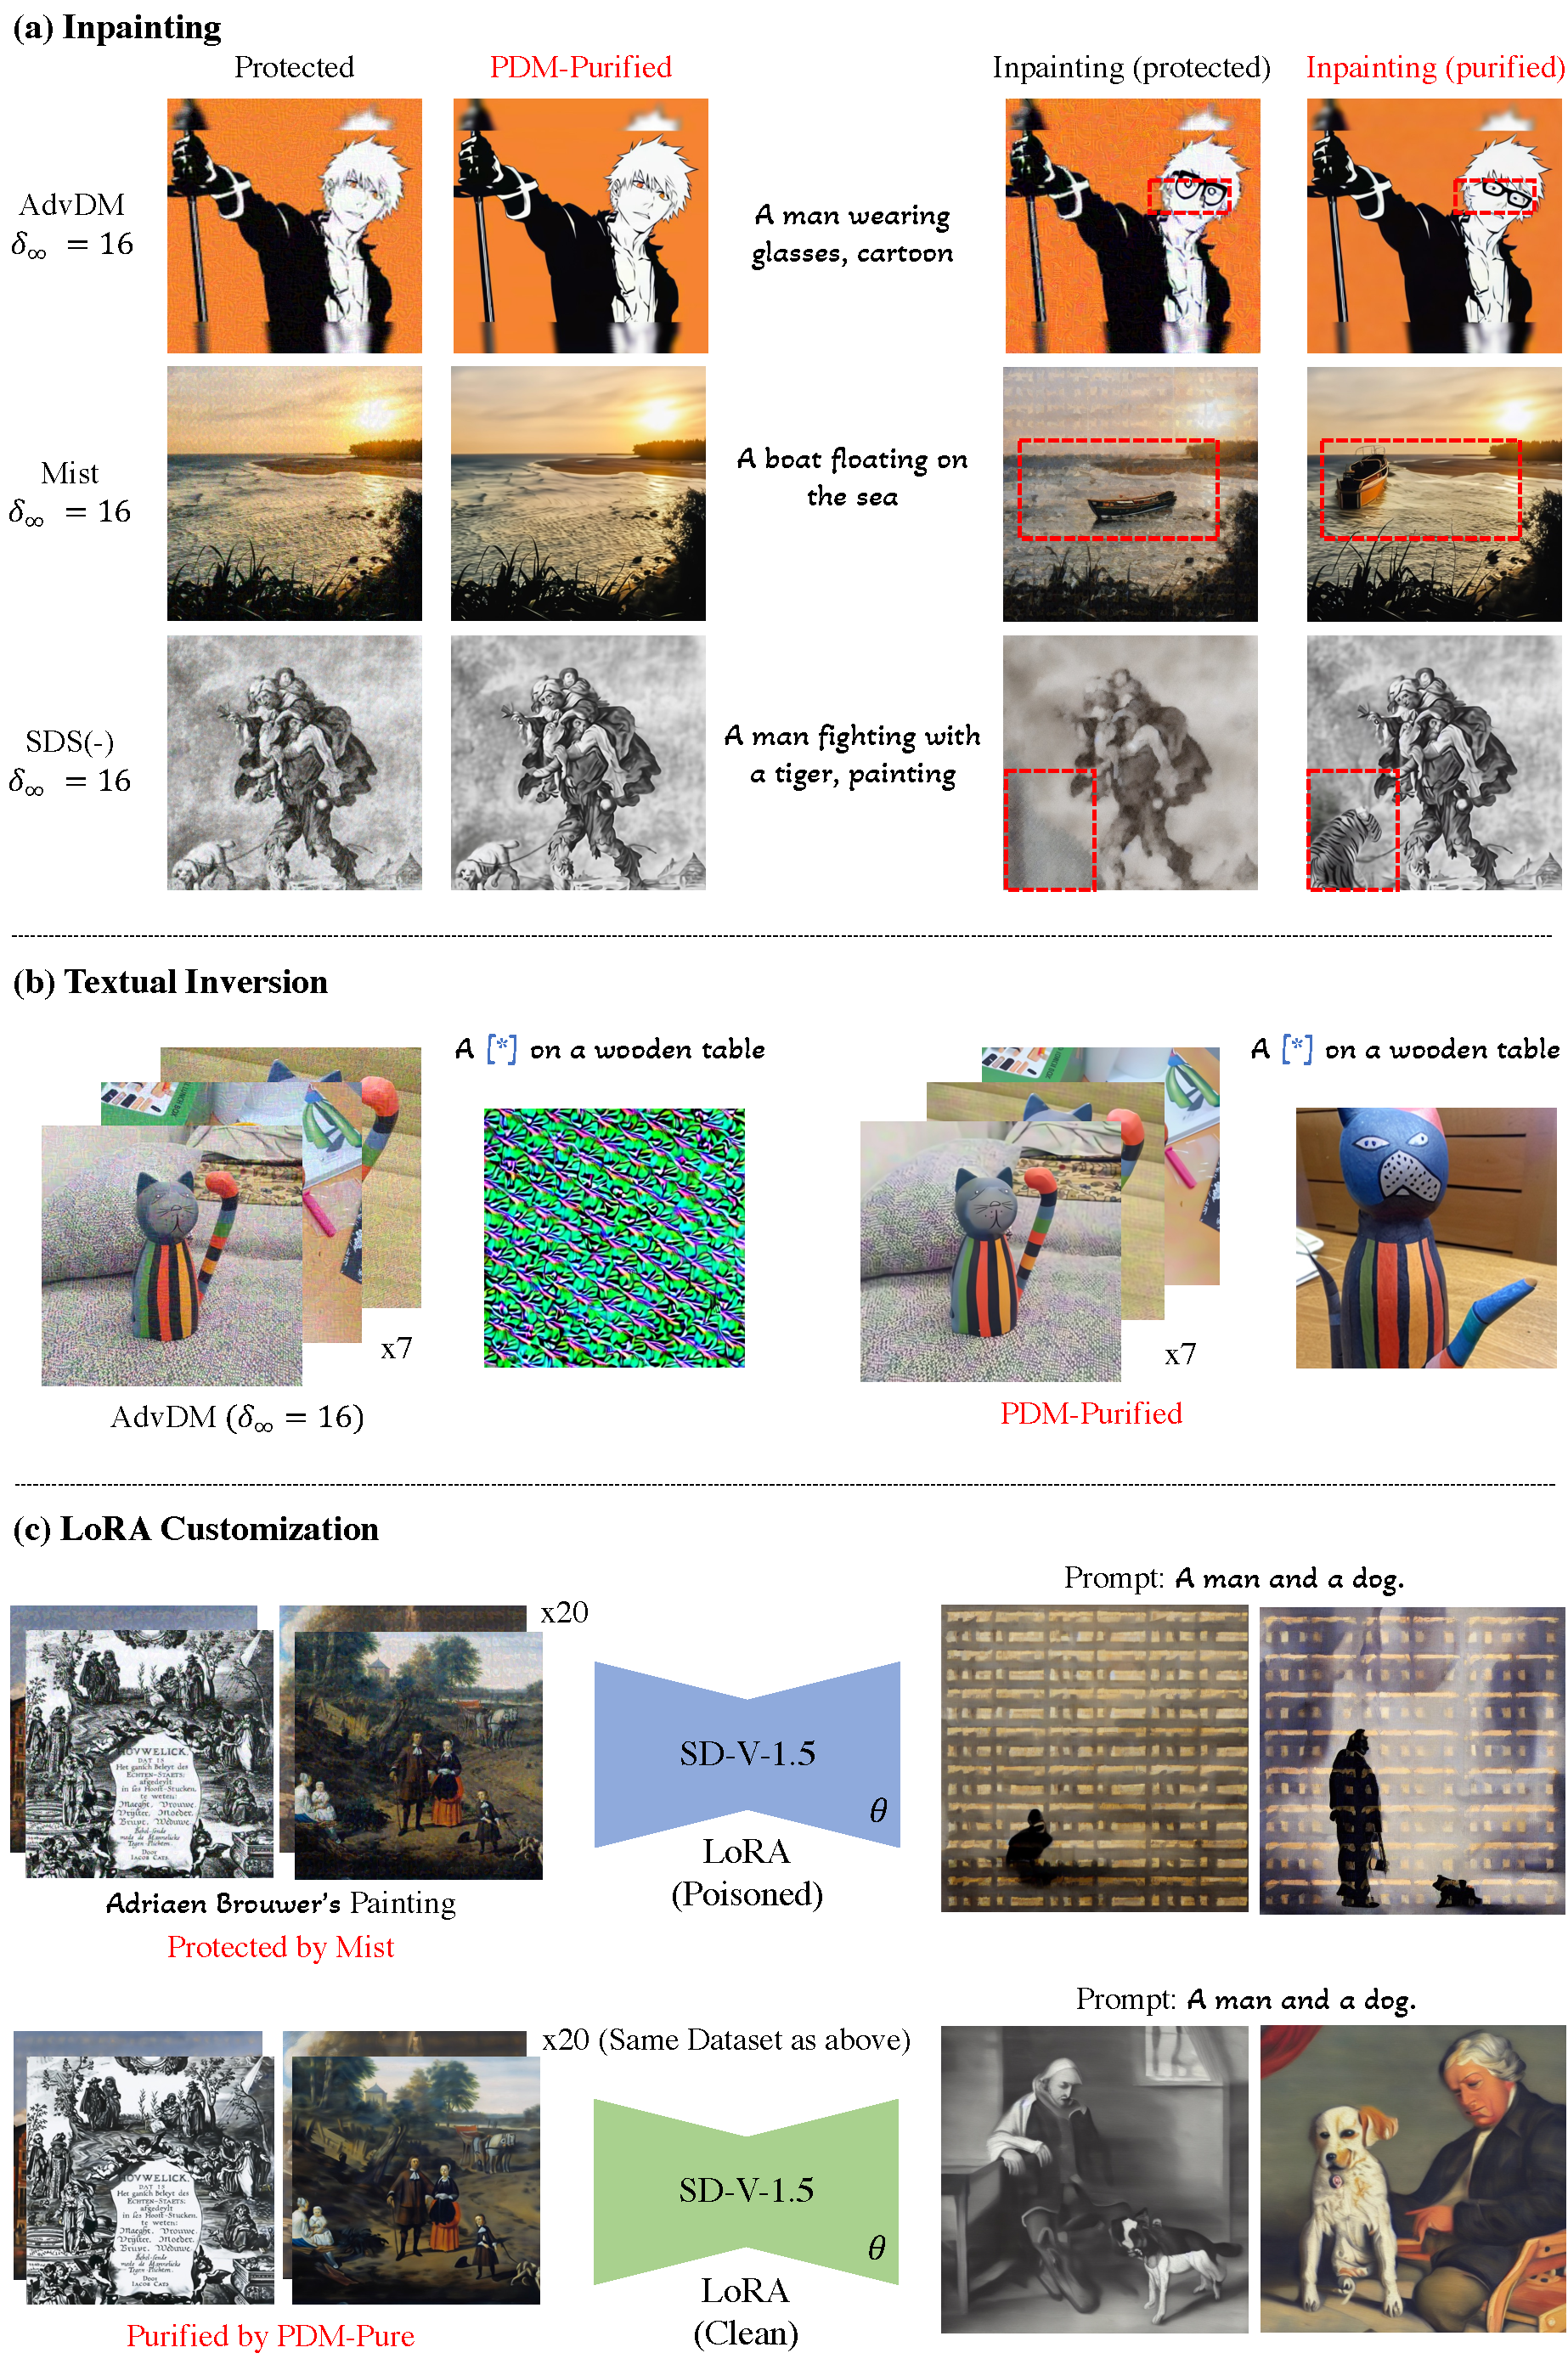
\includegraphics[width=0.99\linewidth]{images/lora.pdf}
  \vspace{-5pt}
  \caption{
  \textbf{PDM-Pure makes the Protected Images no more Protected:} Here we show qualitative results of PDM-Pure on three scenarios where unauthorized editing may occur: (a) Inpainting, (b) Text-Inversion~\cite{textualinversion} and (c) LoRA customization~\cite{lora}. While the protected images incur bad generation quality, the purified ones can fully bypass the protection.
  }
  % \caption{\textbf{Qualitative Results of PDM-Pure in Inpainting:} PDM-Pure can effectively remove the adversarial patterns in various protection methods, here we show image inpainting results on three typical protection methods: AdvDM~\cite{advdm}, Mist~\cite{liang2023mist} and SDS(-)~\cite{sdsattack} on Stable Diffusion V-1.5. We show results on quite strong attacks with budget $\delta_{\infty}=16/255$. We can see the figures are no more adversarial after PDM-Pure, resulting in much better inpainting results. (inpainting regions are indicated by the the bounding boxes; zoom in on screen for better observation)}

  \label{fig:purification_results}
\end{figure}


%% test citation
% \citep{diff-pgd, sdsattack}

{
\small
\bibliographystyle{abbrvnat}
\bibliography{bibliography}
}

\newpage  
\tableofcontents


\newpage
\appendix
\section*{Appendix}
In support of the main paper,~\cref{app:proofs} presents the proofs for the propositions in the paper,~\cref{app:additional_findings} includes additional findings that support our main results, and~\cref{app:further_discussion} provides further discussion on conditions that lead to grokking.
\section{Proofs}\label{app:proofs}
\begin{proof}[Proof of~\cref{prop:stablemax}]
\begin{align}
    \softmax\left(g\left(x_i\right)\right) &= \frac{e^{g(x_i)}}{\sum_j e^{g(x_j)}}\\
    &= \begin{cases}
\frac{e^{\log(x_i+1)}}{\sum_j e^{\log(x_j+1)}} & \text{if } x_i \geq 0, \\
\frac{e^{-\log(-x_i+1)}}{\sum_j e^{-\log(-x_j+1)}} & \text{if } x_i < 0
\end{cases}\\
&= \begin{cases}
\frac{x_i+1}{\sum_j x_j+1} & \text{if } x_i \geq 0, \\
\frac{\frac{1}{-x_i+1}}{\sum_j \frac{1}{-x_j+1}} & \text{if } x_i < 0
\end{cases}\\
&= \stablemax(x_i).
\end{align}
\end{proof}

\begin{proof}[Proof of~\cref{prop:NLMGrad}]
To prove that any nonzero $-\nabla_{\perp} \loss(\bm{\theta}_t)$ is a descent direction, we need to show that $\left\langle -\nabla_{\perp} \loss(\bm{\theta}_t), \nabla\loss(\bm{\theta}_t) \right\rangle < 0$, assuming $\nabla_{\perp} \loss(\bm{\theta}_t) \neq \mathbf{0}$:
    \begin{equation}
        \left\langle \nabla\loss(\bm{\theta}_t), -\nabla\loss(\bm{\theta}_t) + \left( \frac{\bm{\theta}_t^\top \nabla \loss(\bm{\theta}_t)}{\bm{\theta}_t^\top \bm{\theta}_t} \right)\bm{\theta}_t  \right\rangle \leq 0.
    \end{equation}
    Expanding this yields:
    \begin{align}
        -\left\|\nabla\loss(\bm{\theta}_t)\right\|^2_2 + 
        \left\langle  \nabla\loss(\bm{\theta}_t), \bm{\theta}_t \frac{\bm{\theta}_t^\top \nabla \loss(\bm{\theta}_t)}{\bm{\theta}_t^\top \bm{\theta}_t}\right\rangle
        &\leq 0.
    \end{align}
    Since the inequality is unaffected by the scaling of the left hand side, we can, without loss of generality, assume that the gradients are normalized, leading to:
    \begin{align}\label{eq:incidence}
        \left\langle \nabla\loss(\bm{\theta}_t), \bm{\theta}_t \frac{\bm{\theta}_t^\top \nabla \loss(\bm{\theta}_t)}{\bm{\theta}_t^\top \bm{\theta}_t}\right\rangle
        &{\leq} 1.
    \end{align}
    Since $\bm{\theta}_t \frac{\bm{\theta}_t^\top \nabla \loss(\bm{\theta}_t)}{\bm{\theta}_t^\top \bm{\theta}_t}$ denotes the projection of the gradient onto the space spanned by the weights, $\langle\cdot,\cdot\rangle$ will measure the acute angle of incidence and hence~\cref{eq:incidence} holds, with equality iff $\nabla_{\perp} \loss(\bm{\theta}_t) = \mathbf{0}$, which is prevented by assumption. This proves that $-\nabla_{\perp} \loss(\bm{\theta}_t)$ is a descent direction while being perpendicular to the weights. %, the angle between $\loss(\bm{\theta}_t)$ and this projection will be the acute .
\end{proof}
We note that the \ograd stops when $\nabla_{\perp}\loss(\bm{\theta}_t) = \mathbf{0}$. If $\nabla\loss(\bm{\theta}_t) \neq \mathbf{0}$, this corresponds to the condition where the gradient is in the same direction with the parameter vector. $\nabla_{\perp}\loss(\bm{\theta}_t) = \mathbf{0}$ can also be the case if $\nabla\loss(\bm{\theta}_t) = \mathbf{0}$, which corresponds to the loss function being at a local optimum.

\section{Additional Findings}\label{app:additional_findings}


\subsection{Further evidence that SC prevents grokking} \label{app:sc_intervention}
\begin{wrapfigure}[12]{R}{0.38\textwidth}
            \vspace{-0.4cm}
            \begin{center}
    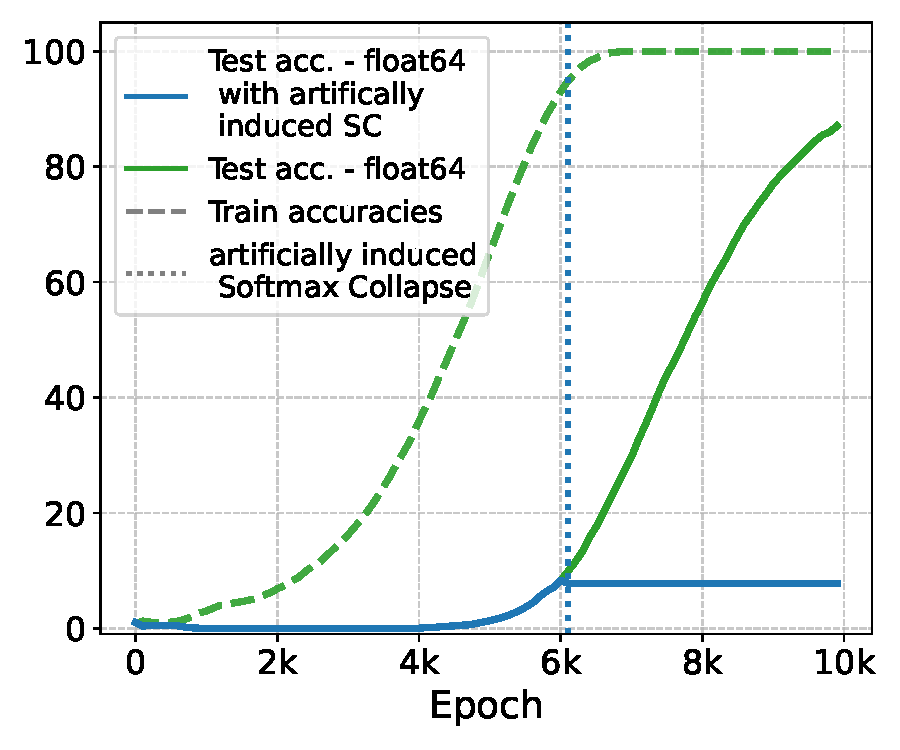
\includegraphics[width=\linewidth]{grokking_iclr_arxiv/figures/artificially_induced_sc.pdf}
            \end{center}
            \vspace{-12pt}
            \caption{Taking a model that would normally generalize (green) and artificially inducing SC has a very similar effect to the one observed in \cref{fig:grokking_stops}.\vspace{4mm}}
    \label{fig:sc_intervention}
\end{wrapfigure} 
While SC leads the gradient from correctly predicted samples to be zero, it does not do this for the incorrect classes. To validate that setting the gradients from the correct classes to zero is enough to stop learning, we do this artificially for a model that is generalizing and show that learning stops after this intervention. In \cref{fig:sc_intervention} we see that the baseline model shown in geen generalizes, but this is stopped at epoch 6000 for the model shown in blue, after we perform this intervention.

The intervention is implemented by multiplying the logits for the right classes by 0 at each step after epoch 6000.

\begin{comment}
\begin{figure}[h]
    \centering
    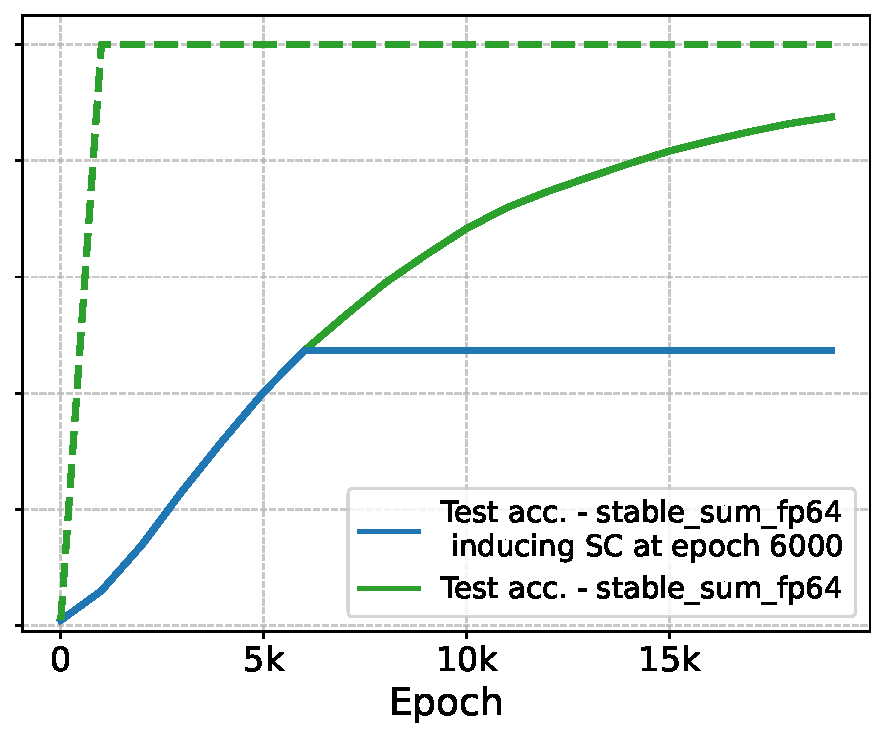
\includegraphics[width=0.5\linewidth]{grokking_iclr/figures/sc_intervention.pdf}
    \caption{Taking a model that would normally generalize (green) and artificially inducing SC has a very similar effect to the one observed in \cref{fig:grokking_stops}}.
    \label{fig:sc_intervention}
\end{figure}    
\end{comment}


\subsection{SGD with learning rate scheduling}
To show that our results are not due to the inductive bias of adaptive moments in optimizers like AdamW, we replicate some of the AdamW results using SGD with a learning rate scheduler. Our scheduler is similar to the one in \cite{Lyu2019-sc} except at each step we divide the learning rate by the norm of the full gradient, instead of the loss. In \cref{fig:grokking_stops_lr_sch} we observe that SC also puts an end to grokking in this setting.
\vspace{5.75mm}\\

\begin{figure}[t]
\centering
\begin{subfigure}{.32\textwidth}
  \centering
  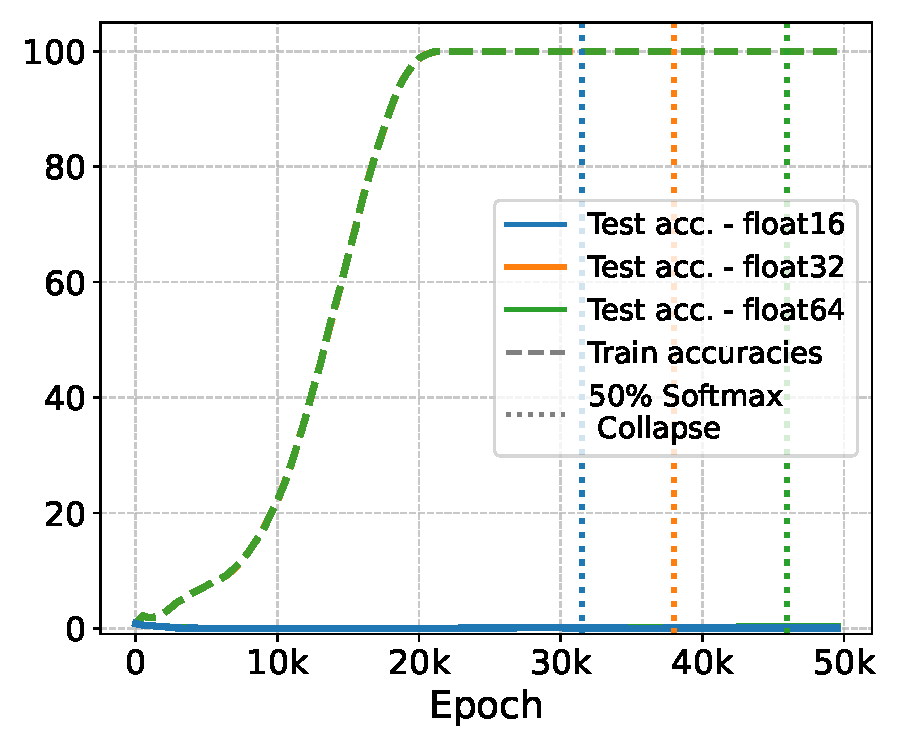
\includegraphics[width=\linewidth]{grokking_iclr_arxiv/figures/float32vsfloat64_40_percent_lr_sch.pdf}
  \caption{40\% training data}
  \label{fig:grokking_stops_40_lr_sch}
\end{subfigure}
\hfill
\begin{subfigure}{.32\textwidth}
  \centering
  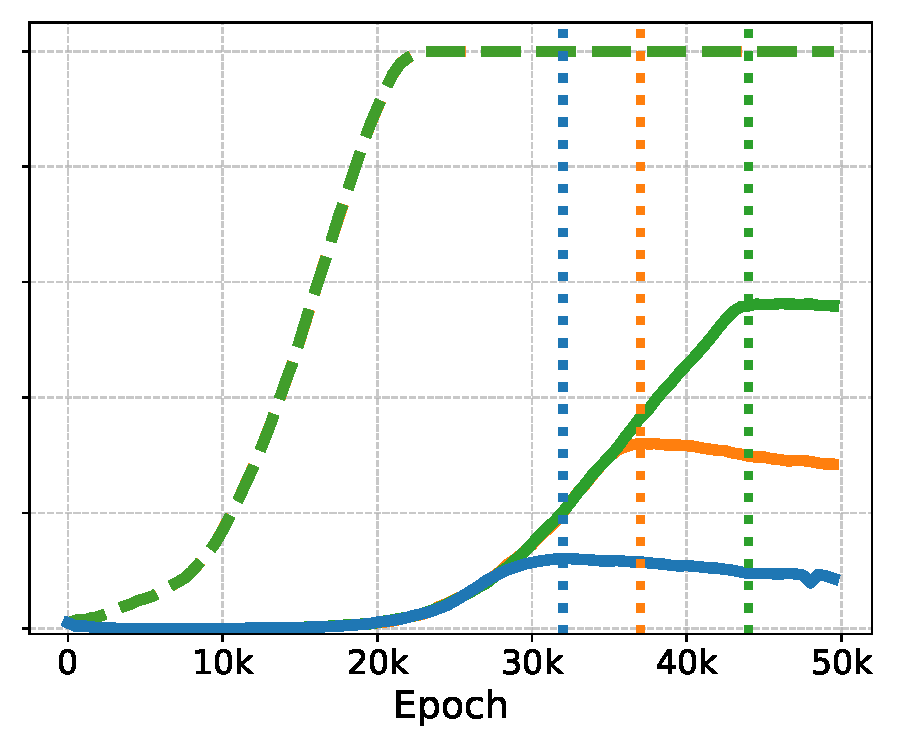
\includegraphics[width=\linewidth]{grokking_iclr_arxiv/figures/float32vsfloat64_60_percent_lr_sch.pdf}
  \caption{60\% training data}
  \label{fig:grokking_stops_60_lr_sch}
\end{subfigure}
\hfill
\begin{subfigure}{.32\textwidth}
  \centering
  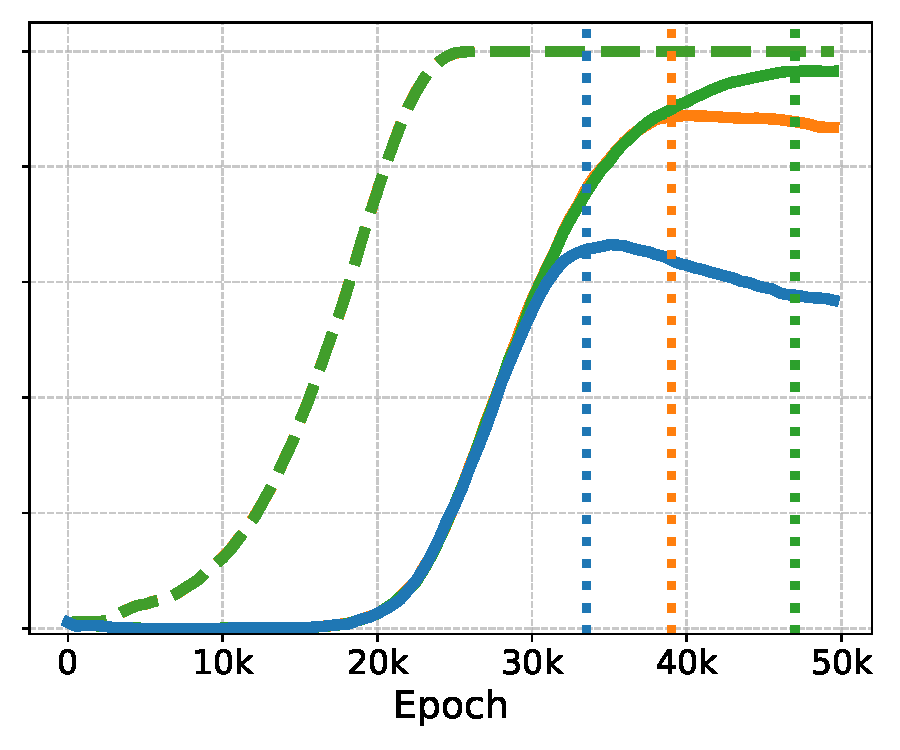
\includegraphics[width=\linewidth]{grokking_iclr_arxiv/figures/float32vsfloat64_70_percent_lr_sch.pdf}
  \caption{70\% training data}
\end{subfigure}
\caption{We show that the same dynamics observed in \cref{fig:grokking_stops} can be observed with a learning rate scheduler instead of AdamW. This shows that this is not due to an implicit bias of adaptive optimizers.}
\label{fig:grokking_stops_lr_sch}
\vspace{-5mm}
\end{figure}

\vspace{-5mm}
\section{Effective Learning Rate}
\begin{wrapfigure}[13]{R}{0.4\textwidth}
            \vspace{-1.2cm}
            \begin{center}
    \includegraphics[width=0.4\textwidth]{grokking_iclr_arxiv/figures/gradient_norms.pdf}
            \end{center}
            \vspace{-10pt}
            \caption{Gradient absorption errors during training on addition modulo 113.}
            \label{fig:gradient_absorption}
\end{wrapfigure} 
Unexplored in the main paper, NLM also has the effect of reducing the effective learning rate. For a gradient update using regular gradient descent $\bm{\theta}_{t+1} = \bm{\theta}_t - \eta \nabla \loss(\bm{\theta}_t)$ it is easy to see that $||\bm{\theta}_{t+1} - \bm{\theta}_{t}|| \to 0$ as $||\nabla \loss(\bm{\theta}_t)|| \to 0$. This problem has been observed before when training beyond the point of overfitting, for example, \cite{Lyu2019-sc} addressed it by using a loss based learning rate scheduler to keep up with the gradient. Theoretically, an alternative could be to simply extend the duration of training. According to our hypothesis, training for long enough should eventually lead to generalization on grokking tasks if we prevent SC. However, we find that another kind of floating point error can also appears in these settings, namely, gradient absorption errors in the weights. 

For a weight $w$, gradient absorption errors happen when a gradient update is small enough that it leaves the weight unchanged. Using the notation outlined in this paper this can be formalised as $w -\eta \frac{\partial \mathcal{L}}{\partial w} \doteq w$. In \cref{fig:gradient_absorption} we show that this happens for an MLP trained with SGD on modular addition using 30\% of the training data. As the norm of the gradient decreases, the percenage of the gradients that are absorbed by the weights increases substantially. Note that the number of gradients that are \textit{exactly} zero remains stable while the number of absorbed gradients increases substantially.

\begin{comment}
\begin{figure}[h]
    \centering
    \includegraphics[width=0.5\linewidth]{grokking_iclr/figures/gradient_norms.pdf}
    \caption{Gradient absorption errors during training on addition modulo 113.}
    \label{fig:gradient_absorption}
\end{figure}
\end{comment}
This issue is naturally mitigated by second order moments for adaptive optimizers like Adam and AdamW which is why they do not frequently appear. However, they do prevent us from showing grokking with vanilla gradient descent without any learning rate schduling. 


\subsection{Additional ways to induce grokking}
Beyond the interventions described in the main text, we highlight two additional ways to induce grokking that validate our hypothesis. 

\paragraph{Logit norm regularization}
Since we argue that uncontrolled scaling of the logits is responsible for delaying grokking and leading to SC, we validate that preventing this scaling of the logits by adding the norm of the logits to the loss, leads to grokking without additional regularization (\cref{fig:additional_grokking_logit}).


\begin{figure}[t]
\centering
\begin{subfigure}{.33\textwidth}
  \centering
  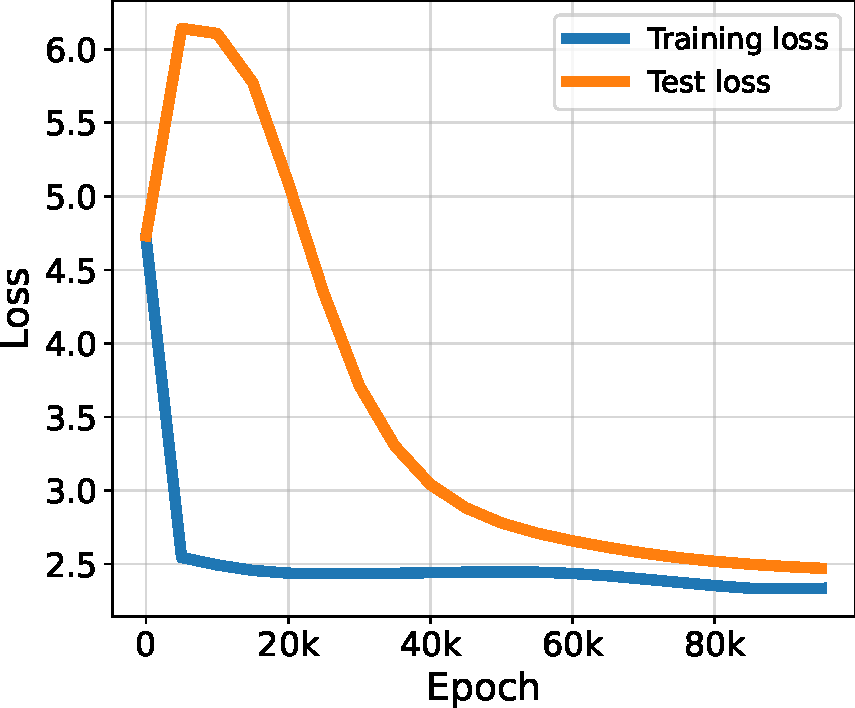
\includegraphics[width=\linewidth]{grokking_iclr_arxiv/figures/softermax_loss.pdf}
  \caption{$\stablemax$}
  \label{fig:additional_grokking_stablemax}
\end{subfigure}%
\hfill
\begin{subfigure}{.33\textwidth}
  \centering
  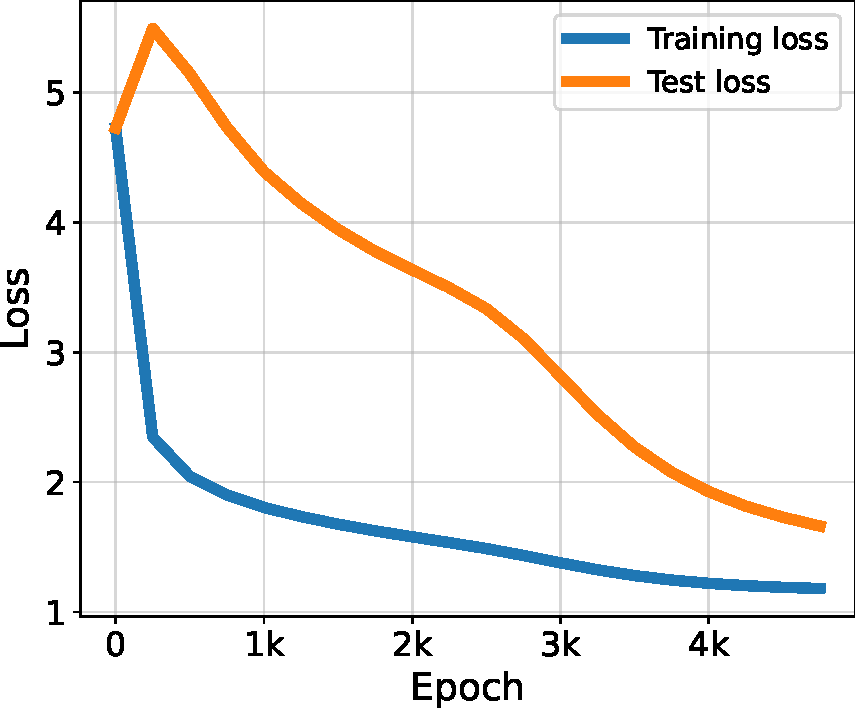
\includegraphics[width=\linewidth]{grokking_iclr_arxiv/figures/logit_reg_loss.pdf}
  \caption{Logit regularization}
  \label{fig:additional_grokking_logit}
  
\end{subfigure}%
\hfill
\begin{subfigure}{.33\textwidth}
  \centering
  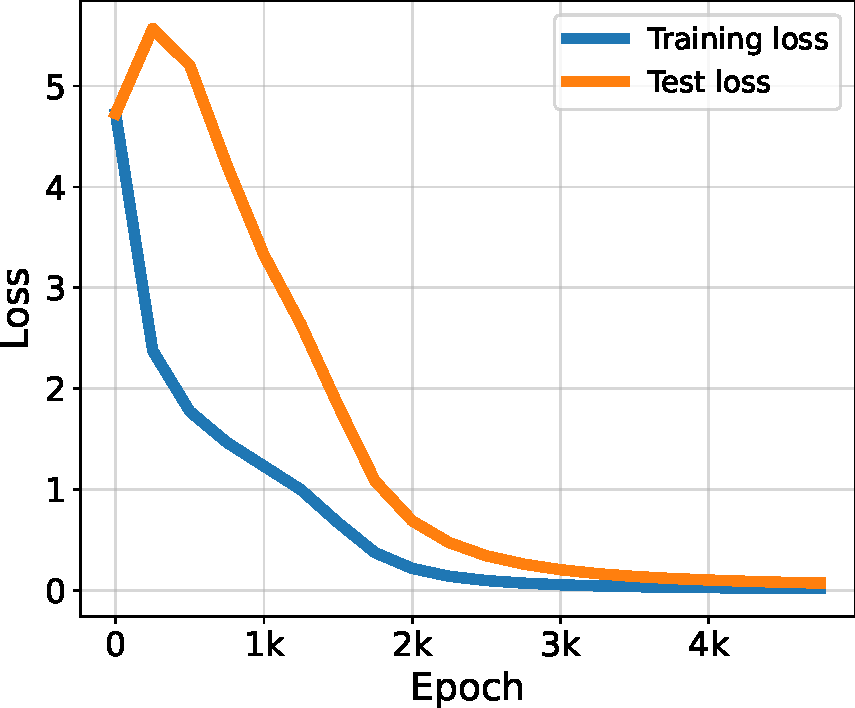
\includegraphics[width=\linewidth]{grokking_iclr_arxiv/figures/taylor_loss.pdf}
  \caption{\tsoftmax}
  \label{fig:additional_grokking_taylor}
\end{subfigure}
\vspace{-3mm}
\caption{Train and test losses during grokking induced by three different interventions.\vspace{-2mm}}
\label{fig:additional_grokking}
\end{figure}

\begin{wrapfigure}[20]{R}{0.4\textwidth}
\vspace{-0.5cm}
    \centering
    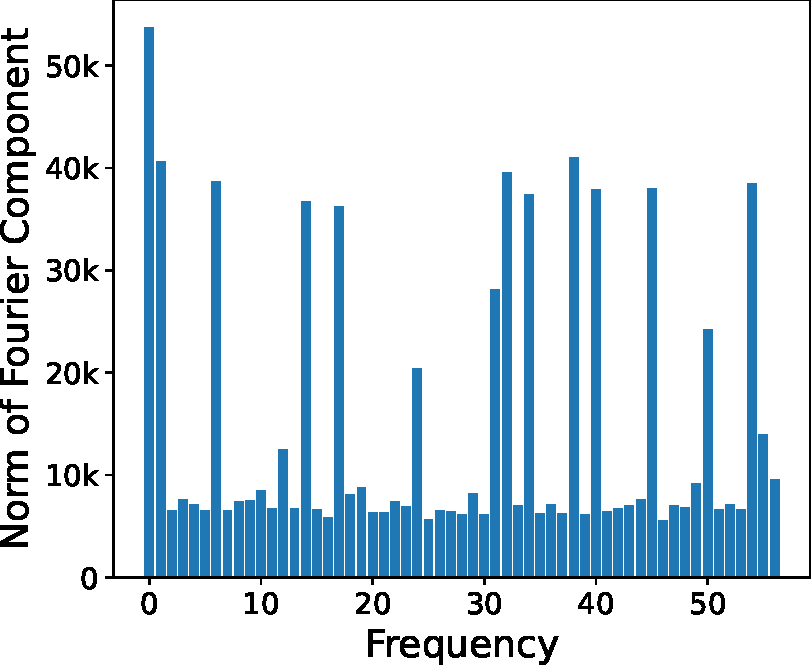
\includegraphics[width=\linewidth]{grokking_iclr_arxiv/figures/fourier.pdf}
    \vspace{-6mm}
    \caption{Fourier components of the weights of the output layer of an MLP trained on addition mod 113. Grokking is induced via $\stablemax$ and without weight decay.}
    \label{fig:fourier}
\end{wrapfigure}
\noindent\textbf{Taylor approximation of the Softmax.}
We have introduced $\stablemax$ as a change to the \softmax that leads to grokking without regularization. The motivation behind this is to prevent values in the sum of the \softmax that are very large or very close to zero. To this end, replacing the exponential with any function that is sub-exponential beyond a certain point should have a similar effect. To demonstrate, we perform a further experiment using the second order Taylor approximation of the exponential 
\begin{equation}
e^x\approx \frac{1 + x + x^2}{2!},    
\end{equation}
replacing the $\exp$ in the \softmax. Since the Taylor approximation is decreasing for $x<0$, we subtract the minimum logit to avoid this part of the function.  We deem this version \tsoftmax.
In \cref{fig:additional_grokking} we see results similar to the ones in \cref{fig:stablemax_grokking} but showing the losses instead of the accuracies as well as results for two additional methods to induce grokking. 
Note that our implementation of \tsoftmax (\cref{fig:additional_grokking_taylor}) introduces an additional implicit regularization similar to the one in  \cref{fig:additional_grokking_logit}, due to the gradient flowing through the subtraction of the mean. % also introduces an additional regularization effect similar to the one 
While this effectively combines the effects of \cref{fig:additional_grokking_stablemax} and \cref{fig:additional_grokking_logit}, leading to grokking faster than the other two methods, our main paper shows results using $\stablemax$ as a cleaner intervention that does not introduce this additional regularization effect. 

% above \tolga{what is the 'one above'?}. This is why we show our main results using $\stablemax$ as a cleaner intervention that does not introduce this additional regularization effect. 

%Note that our implementation of \tsoftmax (\cref{fig:additional_grokking_taylor}) introduces an implicit regularization similar to the one in  \cref{fig:additional_grokking_logit}, effectively combining the effects of \cref{fig:additional_grokking_stablemax} and \cref{fig:additional_grokking_logit}, explaining why it leads to grokking faster than the other two methods. 






\subsection{Solution Learned During Grokking  Without Weight Decay}\label{app:fourier}

\begin{comment}
    \begin{wrapfigure}[20]{R}{0.4\textwidth}
            \vspace{-0.5cm}
            \begin{center}
    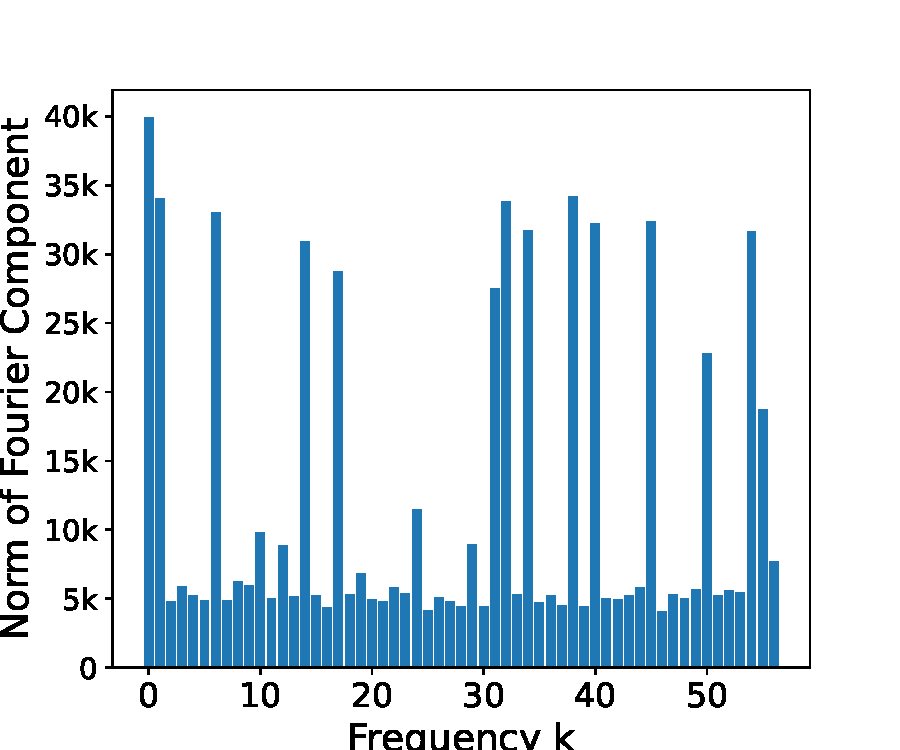
\includegraphics[width=0.4\textwidth]{grokking_iclr/figures/fourier_components.pdf}
            \end{center}
            \vspace{-10pt}
            \caption{Fourier components of the weights of the output layer of an MLP trained on addition mod 113. Grokking is induced with $\stablemax$ and without weight decay. \tolga{this figure is terribly cropped.}}
            \label{fig:fourier}
        \end{wrapfigure}
\end{comment}

 
Weight decay has been identified as potentially responsible for inducing the periodic structures in the weights studied in \cite{Nanda2023-hf}. In \cref{fig:fourier} we show that MLPs that grok without weight decay on modular addition show a similar sparsity in Fourier space as the one observed in \cite{Nanda2023-hf}. While these are very superficial results, they suggest that these structures can emerge without a weight decay--induced ``clean up'' phase as described in \cite{Nanda2023-hf}.

\section{Further Discussion on Conditions that Lead to Grokking}\label{app:further_discussion}
\subsection{L1 regularization and grokking}\label{app:l1_grokking}

%\paragraph{L1 regularization}
While it has been observed that L1 regularization can lead to grokking in some settings, \cite{Nanda2023-hf}
consistently found no grokking with L1 regularization and transformers and this setting has received substantially less attention than weight decay. 

We observe that \nlm scales the weights along their current direction. This means that larger weights are scaled more than small weights. However, while the sign of the gradient from L1 regularization depends on the sign of the weights, the magnitude of this gradient does not depend on the magnitude of the weights. This means that, particularly on deep networks or transformers with with large weights, L1 can sometimes be insufficient to prevent \nlm and the subsequent SC. 
%In Appendix \ref{app:l1_grokking} we show two examples, one where L1 regularization avoids SC and leads to grokking, and one where SC happens despite L1 regularization and grokking does not happen.

\subsection{Delaying generalization by scaling the weights} \label{app:scaling_weights}

\paragraph{Scaling the logits can delay generalization but not induce it} \cite{liu2023omnigrok}, \cite{Kumar2023-hz} and \cite{Lyu2023-ga} showed that an $\alpha$ parameter multiplying the logits can increase or reduce the delay in generalization. We highlight in \cref{fig:alpha_parameter} that this is true for cases where generalization happens even without changing the scale of the logits ($\alpha=1$). However, in most cases when using deeper networks or cross-entropy loss, models do not generalize by default without regularization and we are unable to induce grokking for any value of $\alpha$. 

We argue in \cref{sec:explain_existing_methods} that the observation in \cite{liu2023omnigrok}, \cite{Kumar2023-hz} and \cite{Lyu2023-ga} of grokking without regularization are due to the inductive bias of MSE loss which prevents NLM and leads to grokking in some settings for shallow networks.

\begin{figure}[t]
\centering
\begin{subfigure}{.33\textwidth}
  \centering
  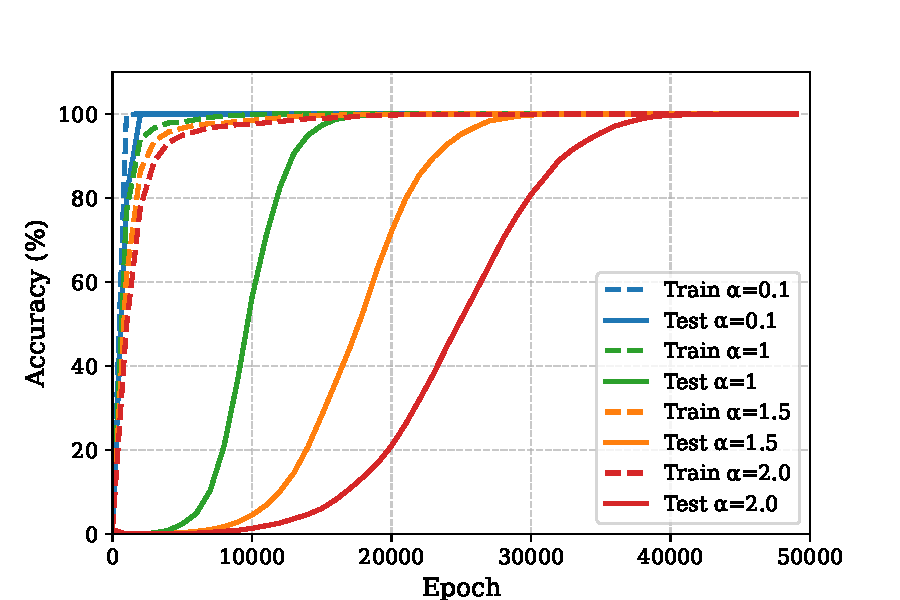
\includegraphics[width=\linewidth]{grokking_iclr_arxiv/figures/one_layer_MSE_alpha_sweep.pdf}
  \caption{MSE: 1 hidden layer}
\end{subfigure}%
\hfill
\begin{subfigure}{.33\textwidth}
  \centering
  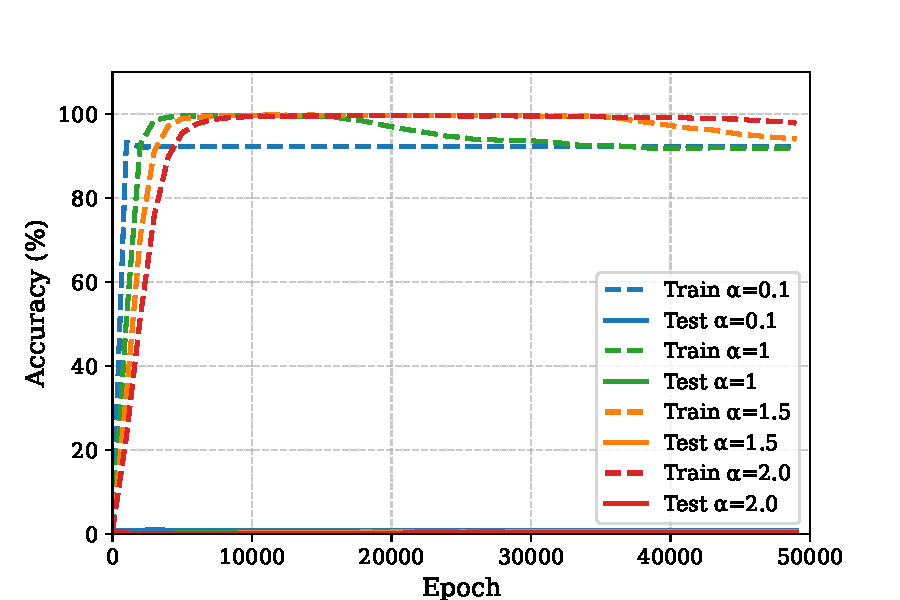
\includegraphics[width=\linewidth]{grokking_iclr_arxiv/figures/two_layer_MSE_alpha_sweep.pdf}
  \caption{MSE: 2 hidden layers}
\end{subfigure}%
\hfill
\begin{subfigure}{.33\textwidth}
  \centering
  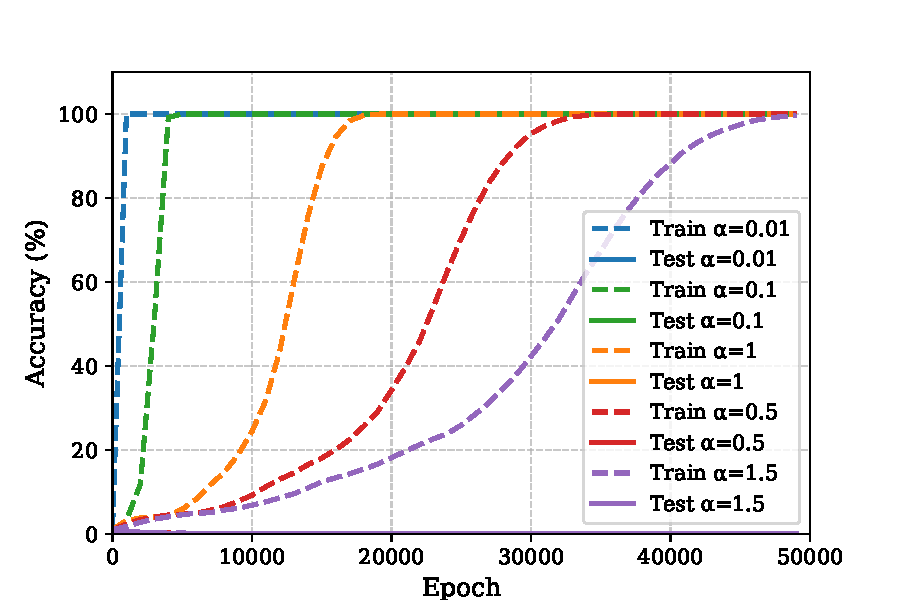
\includegraphics[width=\linewidth]{grokking_iclr_arxiv/figures/two_layer_cross_entropy_alpha_sweep.pdf}
  \caption{CE: 2 hidden layers}
\end{subfigure}
\caption{The $\alpha$ parameter controls generalization in settings where it happens by default. This is the case for shallow networks with MSE loss as shown in subplot (a). However, in deeper networks (b) or networks with CE loss and no regularization (c), $\alpha$ can control the time of over-fitting, but no value of $\alpha$ is enough to trigger grokking.}
\label{fig:alpha_parameter}
\end{figure}

\paragraph{Grokking on MNIST} We replicate the setting from \cite{liu2023grokking} of grokking on MNIST with cross-entropy loss and show that without weight decay, the scaling factor of the weights leads to significant FP errors, preventing grokking from happening until this is alleviated by weight decay. 

While SC explains why weight decay is needed to get the jump in performance observed in \cref{fig:mnist}. It could also explain why inducing grokking by scaling the weights is less effective when using SCE. While when using MSE loss, \cite{liu2023omnigrok} are able to induce full grokking from random level predictions to close to full training accuracy, the same does not seem to be possible when using SCE. In fact, we see in \cref{fig:mnist} that since the begining of training the rate of SC approaches 100\%. This could explain why the observations with cross-entropy loss are not the ones predicted by the lazy training theories outlined in \cite{Kumar2023-hz} which do not take limited floating point precision into account.

\begin{figure}[t]
    \vspace{-6mm}
    \centering
    \begin{subfigure}{.48\textwidth}
    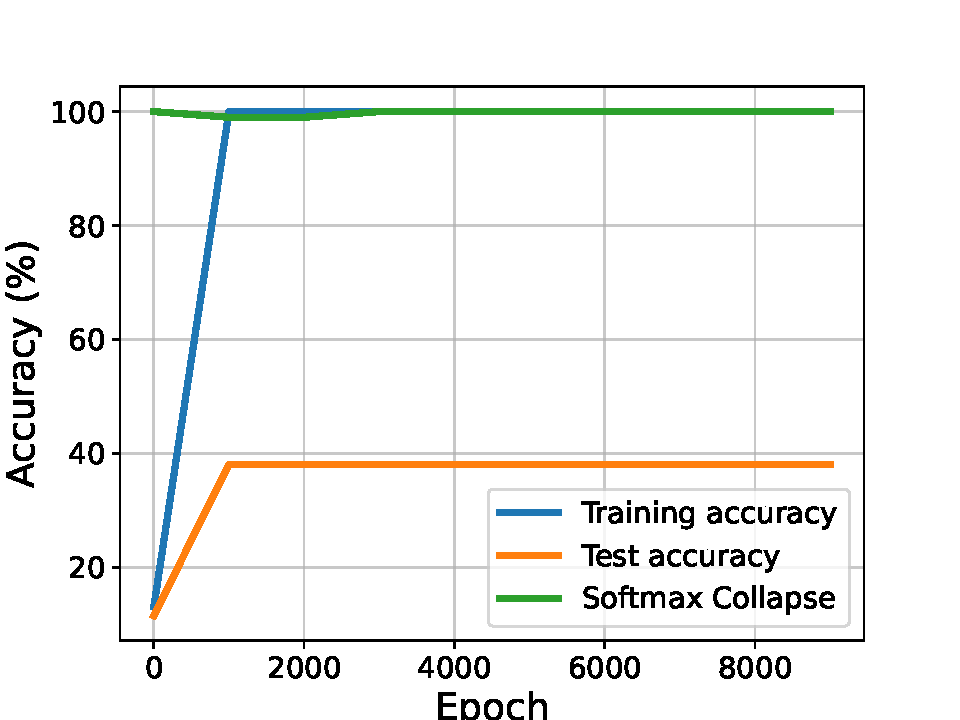
\includegraphics[width=\linewidth]{grokking_iclr_arxiv/figures/mnist_grokking.pdf}
        \caption{MLP without weight decay}
        \label{fig:mnist_witout_weight_decay}
    \end{subfigure}
    \begin{subfigure}{.48\textwidth}
    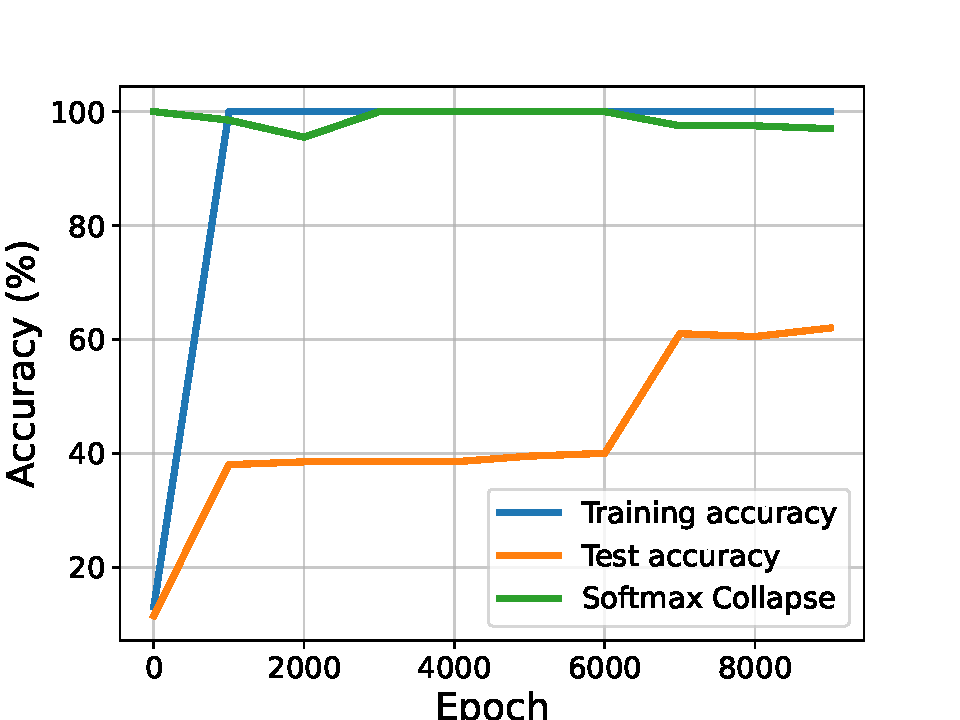
\includegraphics[width=\linewidth]{grokking_iclr_arxiv/figures/mnist_grokking_wd.pdf}
        \caption{MLP with weight decay.}
        \label{fig:mnist}
    \end{subfigure}
    \caption{Replicatting the grokking on MNIST for weight decay setting from \cite{liu2023grokking}. We find that MLPs with weights scaled up by 100 operate at the ``edge of numerical stability'' and in the absence of weight decay, SC eventually reaches 100\%, preventing any further generalization. When using weight decay, the weight norm is reduced, mittigating SC and eventually allowing for further generalization as the SC rate drops from 100\%.}

\end{figure}


\section{\ograd and Weight Decay}
In \cref{fig:wd_vs_ortho}, we provide a more in depth comparison of \ograd and weight decay. \cref{fig:wd_sweep} higlights that increasing the weight decay multiplier leads to a smaller delay in generalization, but only up to a point. In this concrete setting, a weight decay multiplier of 8, prevents the model from fully generalizing (\cref{fig:wd_sweep}). We then compare the best value of weight decay in this setting to \ograd, which does not require any hyper-parameter tuning. \cref{fig:vs_wd_seeds} shows that \ograd leads to faster grokking even when compared to a tuned value of weight decay. Note that the models with weight decay overfit immediately before grokking while \ograd reaches 100\% train and test accuracies almost at the same time.


\begin{figure}[t]
    \vspace{-5mm}
    \centering
    \begin{subfigure}{.48\textwidth}
    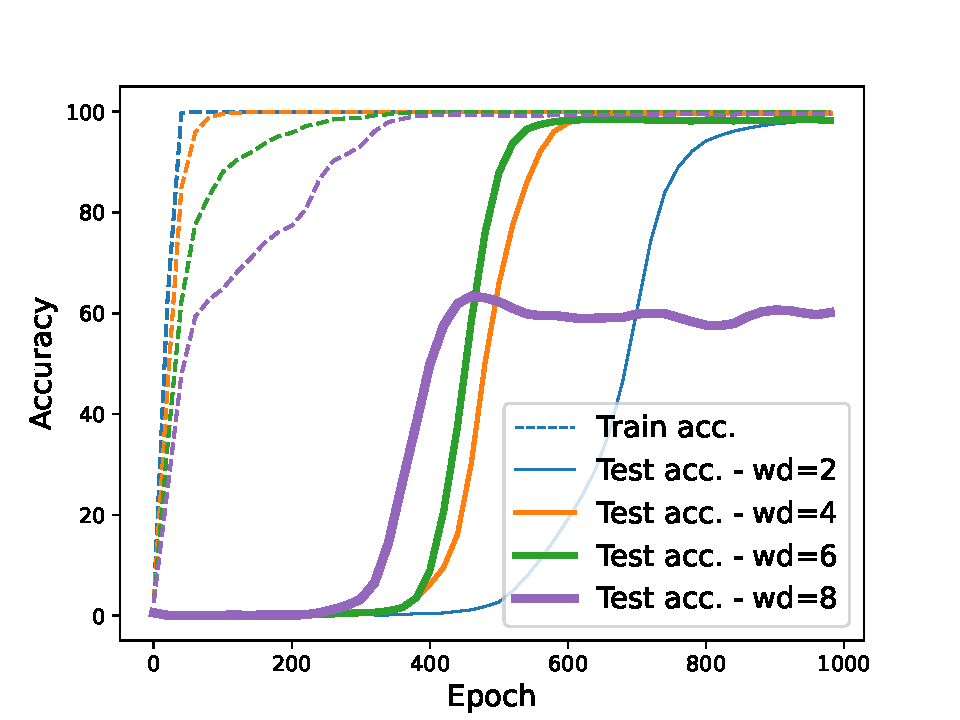
\includegraphics[width=\linewidth]{grokking_iclr_arxiv/figures/weight_decay_sweep.pdf}
        \caption{Sweep over values of weight decay}
        \label{fig:wd_sweep}
    \end{subfigure}
    \begin{subfigure}{.48\textwidth}
    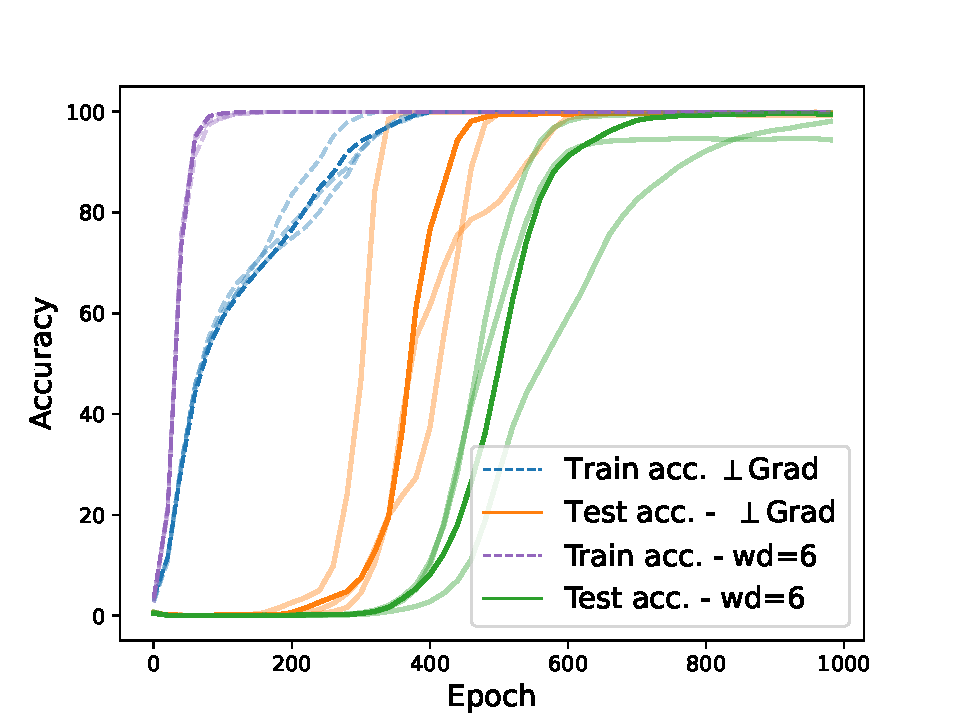
\includegraphics[width=\linewidth]{grokking_iclr_arxiv/figures/weight_decay_vs_orthograd_seeds.pdf}
        \caption{\ograd vs best performing wd model}
        \label{fig:vs_wd_seeds}
    \end{subfigure}
    \caption{Increasing weight decay (WD) for an MLP trained on modular addition with AdamW reduces the delay in generalization up to a point where WD prevents convergence \cref{fig:wd_sweep}. Without any tunable hyper-parameters and without WD, \ograd leads to grokking faster than the best model with WD \cref{fig:vs_wd_seeds}.}
    \label{fig:wd_vs_ortho}
\end{figure}

\section{Alternatives to $\stablemax$ in Preventing SC}
\begin{wrapfigure}[15]{R}{0.45\textwidth}
    \vspace{-7mm}
    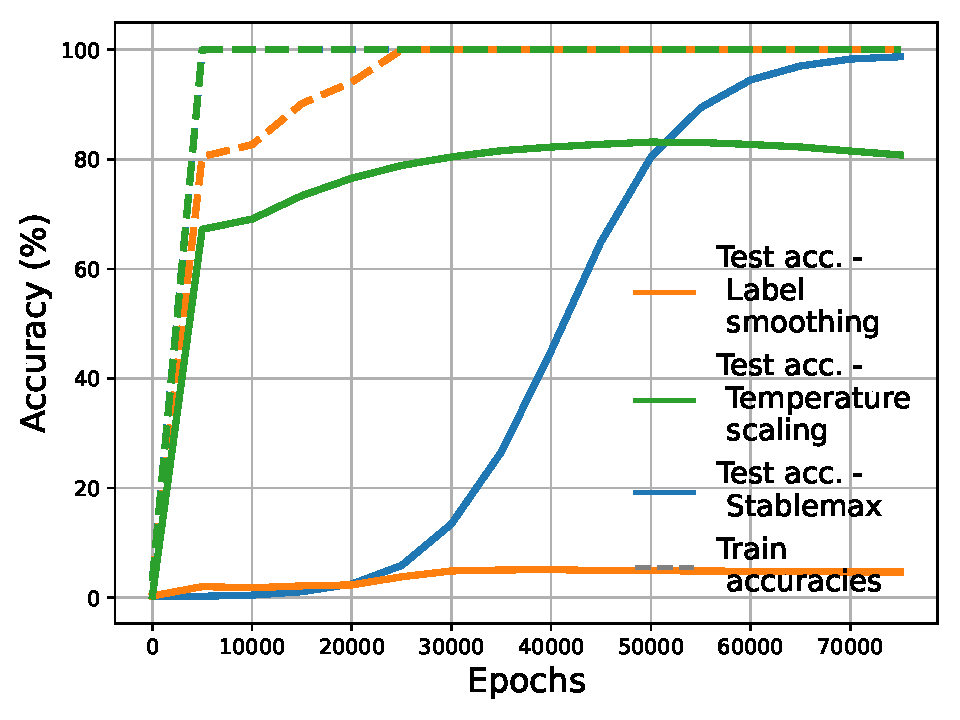
\includegraphics[width=\linewidth]{grokking_iclr_arxiv/figures/label_smoothing.pdf}
    \vspace{-8mm}
    \caption{$\stablemax$ prevents SC and leads to grokking while temperature scaling with $T=1e5$ only gradually delays SC, and label smoothing does prevent SC but at the cost of keeping the model from fully generalizing.}
    \label{fig:label_smoothing}
\end{wrapfigure}
While any intervention that prevents SC should lead to grokking or generalization, \cref{fig:label_smoothing} shows that scaling the temperature of the \softmax is not enough to prevent SC and label smoothing does prevent SC and lead to some generalization, but at the cost of introducing another inductive bias that prevents full generalization and leads to qualitatively different behavior. By comparison, the simple change introduced in Stablemax prevents SC and leads to grokking, serving as a validation for our hypothesis that gradient descent leads to grokking by default, unless this is stopped by SC.



\section{$\stablemax$ and \ograd \\ in Realistic Settings}
While Stablemax and \ograd are designed as interventions to show that preventing SC leads to grokking and preventing NLM leads to generalization (\cref{fig:teaser}), in this section we explore if these methods are applicable in more realistic settings like language modeling with GPT2-small or ResNets trained on image classification. We train GPT2-Small for 1 epoch on WikiText-103 using a batch size of 16, a block size of 512, a learning rate of $5e-4$ and a weight decay of 0.01 using AdamW. The architecture is the regular GPT2-Small architecture from \cite{radford2019language}, trained with a cosine schedule and 1000 steps of warmup.

For CIFAR10, CIFAR100 and Imagenet-1k \citep{ILSVRC15}, our baseline is a ResNet18 with SCE loss trained with SGD 0.9 momentum and $1e-4$ weight decay. We use standard data transformations such as random crop and random horizontal flip and a step learning rate scheduler every 30 epochs for a full training run of 100 epochs. With respect to this baseline we report results replacing the $\softmax$ with $\stablemax$ in the loss function, as well as replacing SGD with $\perp$SGD. Since test labels for Imagenet-1k are not publicly available, we use the validation set as a test set and tune hyper-parameters on a fraction of the training set.


\begin{figure}[t]
    \centering
    \begin{subfigure}{.32\textwidth}
    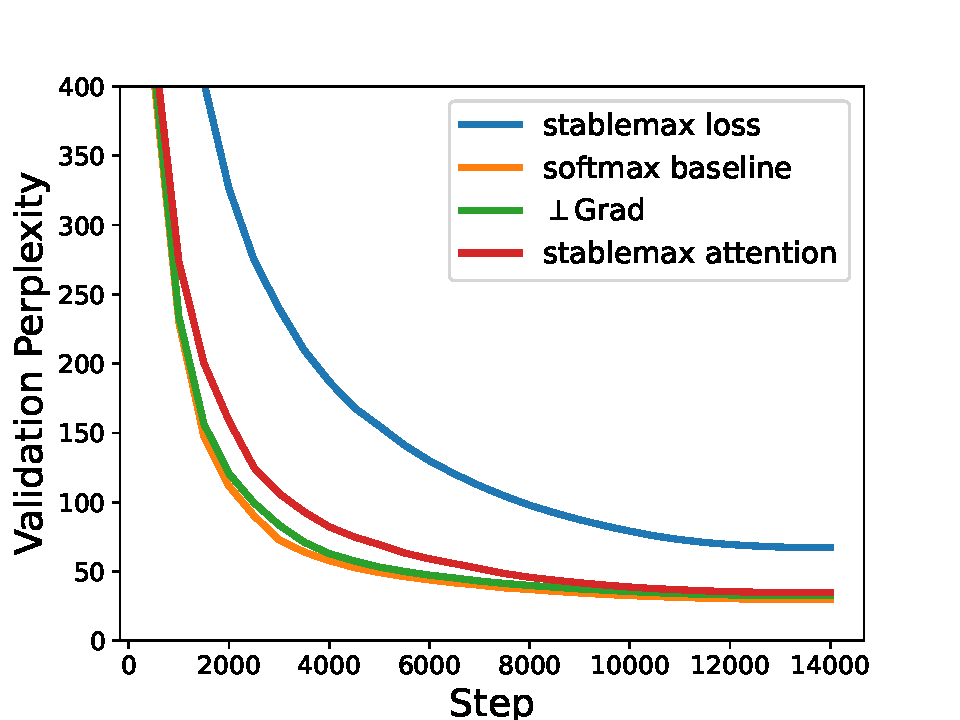
\includegraphics[width=\linewidth]{grokking_iclr_arxiv/figures/gpt2-small.pdf}
        \caption{GPT2-Small on WikiText2}
        \label{fig:gpt2_small}
    \end{subfigure}
    \hfill
    \begin{subfigure}{.32\textwidth}
    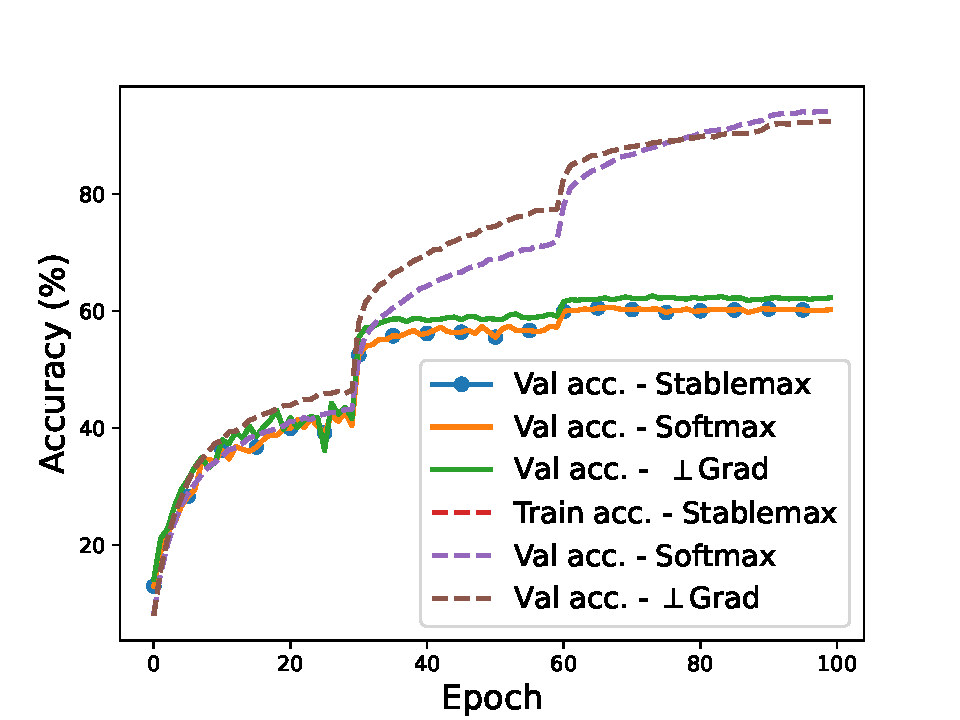
\includegraphics[width=\linewidth]{grokking_iclr_arxiv/figures/CIFAR100.pdf}
        \caption{ResNet18 on CIFAR100}
        \label{fig:cifar100_resnet18}
    \end{subfigure}
    \hfill
    \begin{subfigure}{.32\textwidth}
    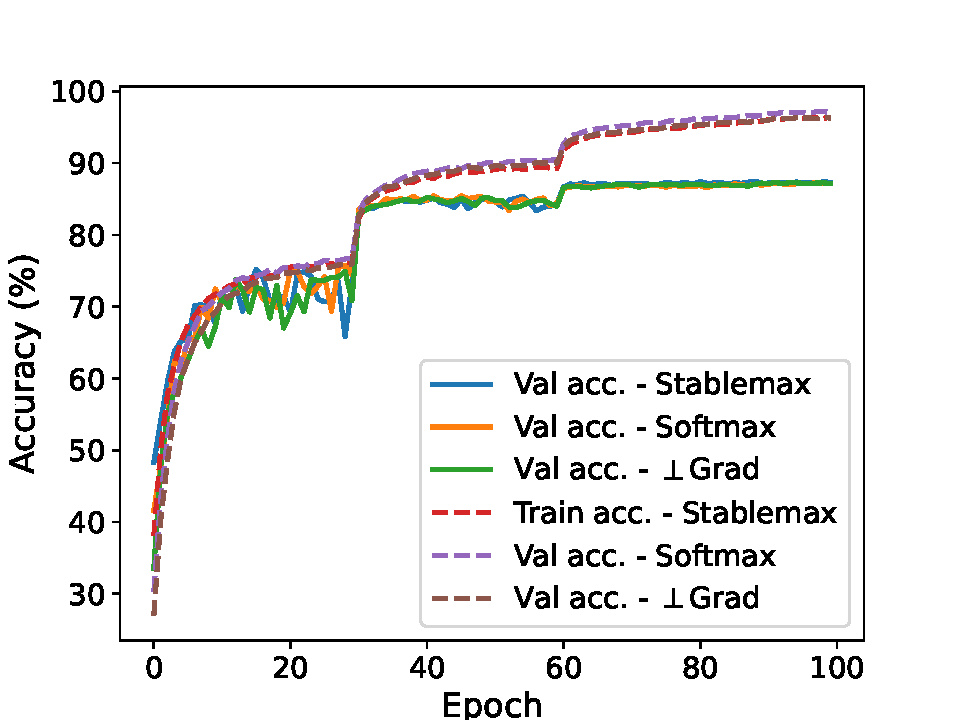
\includegraphics[width=\linewidth]{grokking_iclr_arxiv/figures/cifar10_resnet18.pdf}
        \caption{ResNet18 on CIFAR10}
        \label{fig:cifar10_resnet18}
    \end{subfigure}
    \caption{Comparing Stablemax and \ograd to AdamW with SCE on text data \cref{fig:gpt2_small} and image data \cref{fig:cifar10_resnet18}. For the GPT2-small results in \cref{fig:gpt2_small}, we also include the results of replacing the \softmax in the attention mechanism with $\stablemax$.}
\end{figure}

\begin{table}[h]
\centering
\begin{tabular}{@{}lcccc@{}}
\toprule
\textbf{Method}         & \textbf{CIFAR10} & \textbf{CIFAR100} & \textbf{ImageNet-1k} & \textbf{WikiText-103} (Top-5) \\ \midrule
Softmax CE              & $87.17\% \pm 0.2$ & $59.98\% \pm 0.4$  & $69.33\% \pm 0.04$              & $60.48\% \pm 0.04$                      \\
Stablemax CE            & $87.01\% \pm 0.2$ & $60.63\% \pm 0.4$  & $65.87\% \pm 0.22$             & $51.85\%  \pm 0.47$                  \\
\ograd                  & $87.22\% \pm 0.2$ & $62.69\% \pm 0.1$  & $68.95\% \pm 0.03$               & $59.64\%   \pm 0.04$                \\ 
\midrule
Stablemax Attention     & --                & --                 & --                   & $58.52\%   \pm 0.04$                   \\ \bottomrule
\end{tabular}
\label{tab:realistic_datasets}
\caption{For the methods introduced in this paper, we report accuracies with standard deviations across five seeds for the CIFAR datasets and three seeds for Imagenet-1k and WikiText-103. We report Top-5 accuracy in the case of WikiText-103.\vspace{-3mm}}
\end{table}


\section{SC and the Slingshot Effect}\label{app:slingshots}
\cite{slingshot-mechanism} observed that spikes in the training loss appear when training on grokking tasks with adaptive optimizers like Adam, and that these spikes can lead to generalization without weight decay. Although \cite{Nanda2023-hf} showed that slingshots are not necessary for grokking, it is still unclear what mechanism of adaptive gradient optimizers induces this behavior and why it leads to generalization. In light of the results in this paper, we believe that slingshots could lead to generalization because they prevent full SC. \cite{Nanda2023-hf} pointed out that something like SC could be responsible for these slingshots. One possible mechanism would be that zero gradients for some samples due to SC rapidly diminish the second-order moments leading to a large update or slingshot which moves the model away from full SC, although more research would be needed to properly show this.

While related to our work, slingshots are a different kind of instability which only appears with adaptive optimizers and can allow grokking. In contrast, we identify SC as a very specific issue in the \softmax that can affect any model trained with SCE, not only the ones trained with adaptive optimizers. Additionally SC prevents grokking whereas slingshots can lead to it. Wether and how slingshots are cause by SC remains an open research question, with some supporting evidence from \cite{Nanda2023-hf} which show that slingshots can disappear when using $float64$.

\section{Additional Details About Floating Points}
Beyond our main results, we found that in some cases, grokking could be stopped before SC due to the $\epsilon$ parameter in Adam being too large. While the $\epsilon$ term is designed to give numerical stability to the gradients, in settings with extremely low losses and gradients, the second order moments can be dominated by the $\epsilon$ term, putting an end to learning where it would have continued with a smaller $\epsilon$ value. This echoes the results in \cite{slingshot-mechanism} which shows that increasing $\epsilon$ halts slingshots and grokking, with \cite{Nanda2023-hf} also alluding to the $\epsilon$ parameter being important in some cases.  

Surprisingly, we also found that a simple re-implementation of $torch.nn.functional.log\_softmax$ that does not use the official CUDA kernels can lead the models to keep learning beyond the point where the loss is exactly 0 and some gradients should be 0 with appropriate calculation, outperforming the official implementation for grokking tasks. Learning eventually also stops in this setting and this seems more like a quirk of how gradients are calculated in PyTorch in the absence of an explicitly defined backward pass.




%%%%%%%%%%%%%%%%%%%%%%%%%%%%%%%%%%%%%%%%%%%%%%%%%%%%%%%%%%%%


\end{document}